%%==================================================
%% main.tex for BIT Master Thesis
%% version: 0.1
%% last update: Nov 8th, 2017
%%==================================================

% 默认单面打印 oneside 、硕士论文模板 master

\documentclass[oneside, master]{BIT-thesis-grd}

% 打印选项: 双面打印 oneside;单面打印 twoside
% 模板选项: 硕士论文 master; 博士论文 doctor
\graphicspath{{figures/}}

\usepackage{algorithmic}
%\usepackage[ruled]{algorithm2e}
\renewcommand{\algorithmicrequire}{\textbf{输入:}}  
\renewcommand{\algorithmicensure}{\textbf{输出:}}  
\begin{document}

%%%%%%%%%%%%%%%%%%%%%%%%%%%%%%
%% 封面
%%%%%%%%%%%%%%%%%%%%%%%%%%%%%%

% 中文封面内容(关注内容而不是表现形式)
\classification{TQ028.1}
\UDC{540}

\title{基于超限学习机的半参数自适应控制研究}
\vtitle{基于超限学习机的半参数自适应控制研究}
\author{周浩}
\institute{自动化学院}
\advisor{马宏宾教授}
\chairman{邓志红教授}
\degree{工学硕士}
\major{控制科学与工程}
\school{北京理工大学}
\defenddate{2018年1月}
%\studentnumber{**********}


% 英文封面内容(关注内容而不是表现形式)
\englishtitle{Semi-parametric Adaptive Control Based on Extreme Learning Machine}
\englishauthor{Hao Zhou}
\englishadvisor{Prof. Ma Hongbin}
\englishchairman{Prof. Deng Zhihong}
\englishschool{Beijing Institute of Technology}
\englishinstitute{School of Automation}%School of Automation
\englishdegree{Master of Science}
\englishmajor{Control Science and Enginerring}
\englishdate{January, 2018}

% 封面绘制
\maketitle

% 中文信息
\makeInfo

% 英文信息
\makeEnglishInfo

%打印竖排论文题目
\makeVerticalTitle

% 论文原创性声明和使用授权
\makeDeclareOriginal

%%%%%%%%%%%%%%%%%%%%%%%%%%%%%%
%% 前置部分
%%%%%%%%%%%%%%%%%%%%%%%%%%%%%%
\frontmatter

% 摘要
%%==================================================
%% abstract.tex for BIT Master Thesis
%% version: 0.1
%% last update: Nov 8th, 2017
%%==================================================

\begin{abstract}
本文……。({\color{blue}{摘要是一篇具有独立性和完整性的短文,应概括而扼要地反映出本论文的主要内容。包括研究目的、研究方法、研究结果和结论等,特别要突出研究结果和结论。中文摘要力求语言精炼准确,硕士学位论文摘要建议500$\sim$800字,博士学位论文建议1000$\sim$1200字。摘要中不可出现参考文献、图、表、化学结构式、非公知公用的符号和术语。英文摘要与中文摘要的内容应一致。}})

\keywords{超限学习机;半参数;估计;自适应控制}
\end{abstract}

\begin{englishabstract}

   In order to exploit …….
   
\englishkeywords{Extreme learning machine; Semi-parametric; Estimation; Adaptive control}

\end{englishabstract}


% 加入目录
\tableofcontents

% 加入表格索引
%\listoftables

% 加入插图索引
%\listoffigures

%%%%%%%%%%%%%%%%%%%%%%%%%%%%%%
%% 正主体部分
%%%%%%%%%%%%%%%%%%%%%%%%%%%%%%
\mainmatter

%% 各章正文内容
%%==================================================
%% chapter1.tex for BIT Master Thesis
%% version: 0.1
%% last update: Nov 8th, 2017
%%==================================================
\chapter{绪论}
\label{chap:intro}
\section{本论文研究的目的和意义}%\label{sec:***} 可标注label

自动控制理论的进步和发展意味着动态系统的性能更优,意味着生产力的提高,或者意味着自动化程度的提高等,因此自动控制在工程和科学领域一直都起着至关重要的作用。自动控制的基本思想甚至可以追溯到公元前300年左右\upcite{CLiZhuLi2004},其理论的初步形成源于在二十世纪中叶奈奎斯特、伯德、维纳等人建立的经典控制理论,其建立在频率法和根轨迹法等方法的基础上;1960年左右,Kalman 等人提出的状态空间方法与概念标示着现代控制理论与方法的萌芽和诞生。而后,自动控制系统的运行环境越来越复杂,人们对系统控制的目标越来越多,要求也越来越苛刻。随着科学技术的发展和应用需求的不断催生,加上众多学者的不断努力,基于状态空间、传递函数等反馈理论基础和实践过程,现代控制理论迅速兴起。近年来,不论是在现代工业领域,还是在国防科技领域,现代控制理论都发挥着举足轻重的作用。线性系统理论、系统辨识理论、最优控制理论、自适应控制理论和鲁棒控制理论等重要分支的蓬勃发展,促进了自动控制在机器人伺服系统、工业过程、航空航天、人口与经济控制等领域的应用。

在经典控制理论和现代控制理论中,通常假设被控对象是线性系统并且模型的参数是精确已知的,然后以此为前提设计控制律。典型的控制方法\upcite{Katsuhiko2005,Pan1990}就是比例-积分-微分(PID)控制、极点配置\upcite{BraschPearson1970}、线性二次型调节器等。其中针对单变量的PID反馈控制算法应用十分广泛,到目前为止,工业过程大部分也都采用PID控制或者其改进算法。实际系统从本质上来说都是非线性的,而非线性系统的表现形式丰富多彩,比如饱和、时滞、间隙、死区等;对这些的复杂非线性系统, 目前没有很好的系统辨识方法和实际测量工具能够给出系统精确的建模结果,对系统认知的有限性和对系统模型不精确描述,造成系统普遍存在一定的不确定性;许多系统例如机器人、飞行器等运动控制系统都是强耦合的,增加了系统的不确定性。系统的非线性(nonlinearity)和不确定性(uncertainty)给分析和设计控制律带来了极大的挑战。一方面,由于系统工作环境和时间累积的影响,系统实际模型的参数和标称模型的参数总会存在不确定的误差,系统的负载和惯量也会在长时间运行之后发生变化,这些因素都导致了系统参数的不确定性,不恰当的处理会导致系统性能的降低,甚至引起系统的不稳定。另一方面,系统中可能存在的未建模动态、执行器的非线性特性等,也会影响系统的性能,如摩擦非线性会引起伺服系统在低速运转下的不平稳,出现时滞现象;而输入间隙、死区则容易导致系统出现抖震和极限环。因此作为影响系统控制性能的重要因素,与系统不确定性特别是非线性系统的不确定性相关理论研究和实际运用一直备受关注。

随着计算机技术、网络技术的飞速发展,越来越多的控制系统采用数字微处理器作为控制器,特别是机器人伺服系统、航空航天控制系统等运动控制领域。数字化和网络化是现代伺服电机和飞行控制器等的发展趋势。机器人和飞行器等本体作为被控对象,从本质上来说都是连续时间系统,而给这些被控对象施加的都是离散控制信号,只是采样时间很短,通常在毫秒级别。为了简化,在给这些系统设计控制律的时候,常常借助于连续时间控制理论去设计,然后直接施加离散时间控制信号。这样的手段在使用过程中一般不会出现问题,但是存在着隐患,因为系统离散化后特性常常发生变化,也就是输入输出关系发生了改变,特别是非线性和不确定性等特性经过离散化变得更加不可预测。例如,摩擦、死区等非光滑非线性经过离散化之后,更加难以用数学模型精确描述或近似,增加了系统的不确定性。如果不加考虑,可能会使得系统不稳定。因此,从离散时间角度研究实际系统的控制问题更加符合真实条件。

本文将上述的非线性、不确定性和离散化导致的未知因素统一归纳为参数不确定性(parametric uncertainty)和非参数不确定性(non-parametric uncertainty)随着控制理论的不断发展,对非线性系统的不确定性的处理方法也越来越多,如 鲁棒控制、自适应控制等。在这些方法中,自适应控制基于其完善的理论基础和良好的鲁棒性能,在系统不确定性的相关研究中起着极其重要的作用。自适应控制在线性系统中的应用相对来说已经比较成熟,基于连续时间对象的自适应控制算法也层出不穷。然而针对同时具有参数不确定性和非参数不确定性的离散时间自适应控制相关研究还处于探索阶段。本文将借鉴一些其他领域的思想,如机器学习、数据驱动、先验知识关联、计算几何等,同时解决存在这两种不确定性的系统控制问题,这一方向的研究具有相当大的理论意义和实用价值。

\section{国内外研究现状及发展趋势}%\label{sec:***} 可标注label

\subsection{自适应控制}%\label{subsec:***} 可标注label

一般认为,自适应控制的相关理论和技术起源于二十世纪五十年代解决不同飞行高度飞行器的控制器设计问题。自适应控制是在指在被控对象的参数未知或者时变的情形下,在常规反馈控制器中引入自适应算法,动态地对控制方案进行调节,以抵消被控对象的模型时变或受到较大干扰的影响。线性系统的自适应控制方法已经比较成熟,在解决线性被控对象在参数未知和时变情形下取得了比较满意的控制效果。自适应控制的核心思想在于对系统不确定性进行估计、辨识和学习,同时设计出稳定的控制律,这使得控制器能满足系统的实际情况。辨识与控制的具体设计是实现自适应估计与控制哲学的关键步骤。模型参考自适应控制(Model Reference Adaptive Control, MRAC)和自校正控制(Self-tuning Control, STC)是解决线性系统的两类典型自适应控制方法。除了这两种写入教科书的经典自适应控制方法外,经过数十年的发展,还涌现了自适应PID整定、特征模型全系数自适应控制、集值系统自适应控制、L1-自适应控制、无模型自适应控制、模糊自适应控制等\upcite{MaZhangZhou2016}。

除了自适应控制,在解决系统的不确定性问题时,鲁棒控制也是一种比较常用的方法。鲁棒控制方法指的是设计一种控制器,使得当系统存在一定程度的参数不确定性和未建模动态时,闭环系统仍能保持稳定,并保持一定的动态性能\upcite{BallCohen1987}。一般来说,鲁棒控制器的设计和最终效果都依赖于对系统不确定性程度的先验假设。为了使系统稳定,常常假设系统的不确定性在较小的范围内,并且鲁棒控制器设计过程中某些项的对消或者抑制等也严格利用了系统的假设结构和精确的先验知识,这样导致鲁棒控制不能解决系统存在较大不确定性的情形。相对于鲁棒控制,自适应控制由于在反馈回路中嵌入了在线学习机制,因此能够对付较大的系统不确定性。

针对非线性特性或者非参数不确定性的辨识方法常常是设计出性能满意的自适应控制律的难点,特别是对于现代数字化控制器,在被控对象的数据经过离散采样化之后系统对应的结构和参数都存在较大不确定性。虽然经典的控制理论是从连续时间系统的研究出发,并且现代控制理论很多也是基于连续时间对象考虑的,并且在许多实际应用中取得了比较好的控制效果。但是,模拟量连续控制器由于扩展性和可重构性差,且设计复杂的控制规律时十分复杂,随着计算机技术的发展逐渐被历史淘汰。相反,数字化和离散化控制器越来越被广泛应用。实际的被控对象是离散时间系统,这样从连续时间角度设计的控制器嵌入到实际过程中形成闭环系统后,与理论分析有较大偏差,这必然会限制实际的控制性能的提高。

经典的模型参考自适应控制主要针对连续时间系统建立。自校正控制从一开始就是针对离散时间系统而建立的自适应控制规律,即可考虑如下被控对象
\begin{equation}%
\label{eq:ARX}
y_{k+1} = \theta^{T} \phi_{k} + \omega_{k+1}
\end{equation}
其中,$u_{k}$,$y_{k}$在$k$时刻的系统输入和输出;$\phi_{k} = [y_{k},y_{k-1},\ldots,\y_{k-p+1},u_{k},u_{k-1},\ldots,u_{k-q}]^{T}$;$p$和$q$分别是系统输出和输入的阶数;$\theta$是待估计的参数;$\omega_{k}$是干扰。对于\eqref{eq:ARX}这样的被控对象,使用最小二乘算法(Recursive Least Squares, LS)去辨识未知参数$\theta$,或者递推最小二乘算法(Recursive Least Squares, RLS)\upcite{ChenGuo1991}及其诸多变体,如带遗忘因子的最小二乘算法\upcite{Guo1992}。在解决实际问题时,自校正控制采用参数辨识和必然等价原理设计自适应控制律,这是一种比较容易理解的思路。最小二乘算法主要针对线性系统设计,因而导致经典的基于LS的自校正调节器\upcite{GoodwinRamadge1980}难以对付强非线性的被控对象,相关对比实验也表明了从线性系统角度出发设计的自适应控制在碰到存在具有强非线性的不确定性系统时的捉襟见肘\upcite{MaLum2009}。这常常表现为系统的跟随性能满足不了要求,系统输出与期望存在较大偏差,或者系统难以对付较大的非线性干扰。不过,传统自校正控制算法设计中的必然等价原理对后续的自适应控制器的设计有很好的指导意义。

上述讨论的模型\eqref{eq:ARX}常常被称为带外部输入的自回归模型(auto-regression model with extra input, ARX)\upcite{ChenZhao2014},其中的未知参数向量$\theta$刻画了系统的不确定性,但只是考虑到了参数不确定性。另一种模型被称为Nonlinear ARX(NARX)模型,其单输入单输出情形的方程为
\begin{equation}%
\label{eq:NARX}
y_{k+1} = f(y_{K},y_{k-1},\ldots,y_{k+1-p},u_{k},u_{k-1},\ldots,u_{k-q})+\omega_{k+1}
\end{equation}
和\eqref{eq:Guo}类似,其中$f(\cdot)$为未知非线性函数。方程\eqref{eq:NARX}从非线性的角度刻画了系统的不确定性,将系统当作一个几乎可以说是黑箱的模型,完全不受限与系统的具体机构,直接建立系统输入输出的对应关系。除了随机干扰之外,\eqref{eq:NARX}整个系统的不确定性主要体现在未知函数关系$f(\cdot)$上,显然其囊括了线性过程\eqref{eq:ARX},似乎可以当作一种通用的模型回答之前的问题。然而,要解决好系统\eqref{eq:NARX}的自适应控制问题十分困难,有赖于较好的非线性辨识方法和基于辨识结果设计出合适的控制输入$u_{k}$的表达式,这就涉及到非线性离散时间自适应控制。现代非线性离散时间自适应控制方法\upcite{Li2010,Hou2006,YangDaiLee2009}也都大多针对满足一定简化条件的非线性模型或者某一特定的被控对象进行研究,针对不同的结构采用不同的方法,设计和分析都比较复杂,且通用性较差。

解决具有较大不确定性的非线性系统时,难以找到合适的参考模型与之对应以及难以满足匹配条件,就难以实施模型参考自适应控制方法。从必然等价原理出发实施自适应控制需要解决非线性系统的辨识(identification)与估计(estimate)问题。辨识高阶复杂的受控对象模型依赖于很好的辨识算法,并且,高阶复杂的系统辨识容易导致高阶复杂的控制器,而高阶复杂的控制器会给控制技术的具体实施、诊断维护、成本控制等带来一系列困难。有一些基于数据驱动的自适应控制避开了这个问题,例如,无模型自适应控制\upcite{Hou2014}依据系统的输入输出数据设计控制律,充分利用了数据驱动的思想,不过其算法依赖于动态线性化数据模型的准确性,其假设模型具有局限性。综上所述,在伺服电机、机器人、飞行器等具有强非线性、强耦合的离散时间被控系统中,未知参数、非线性干扰、控制离散化带来的不确定性等这些问题并得到没有很好的解决。

设计上述被控对象的自适应控制器的难点在于如何解决同时存在被控系统的参数不确定性和非参数不确定性\upcite{YangChaiZhai2009}。运动控制系统在高速或者超低速等情况下往往具有很大的不确定性,需要自适应反馈,诸如此类。近年来,郭雷院士等学者\upcite{XieGuo1999}指出自适应反馈机制是存在极限的。受自适应反馈机制的最大能力和局限这一研究方向的启发,马宏宾等学者\upcite{MaLum2009}引入基于集合的辨识方法和数据驱动的思想,归纳出了一种等价模型,即半参数系统(semi-parametric system)用来刻画大部分非线性离散时间对象,由此提出了半参数自适应控制这一研究方向。相比于前面提到的常见自适应控制算法,半参数自适应控制出发点具有独特性,和常见的自适应控制算法的详细比较见表\eqref{tab:adaptive}。半参数自适应控制这一研究方向结合了先验知识和数据驱动的思想,设计思路不依赖于具体的被控对象,是一种比较新颖的思路。目前半参数自适应控制中的非线性部分辨识主要考虑采用的是最近邻估计(nearest-neighbor estimate),这种方法未必最优,可以引入其他非线性辨识方法作进一步的优化和扩展。半参数自适应控制目前正处于探索期,还有待于深入和推广。

\begin{table}\centering
\caption{常见自适应控制算法比较}\label{tab:adaptive}
\begin{tabular}{|c|c|c|c|}\hline
算法名称 & 时间特性 & 适用对象 & 系统不确定性类别 \\ \hline
模型参考自适应控制 &  大部分为连续时间 & 线性系统 & 参数不确定性\\ \hline
自校正调节器 &  大部分为离散时间 & 线性系统 & 参数不确定性\\ \hline
无模型自适应控制 & 大部分为离散时间  & 非线性系统 & 非参数不确定性\\ \hline
半参数自适应控制 & 离散时间  & 非线性系统 & 参数和非参数不确定性\\ \hline
\end{tabular}
\end{table}

\subsection{非线性估计与神经网络}%\label{subsec:***} 可标注label

通常的自适应控制主要处理在控制科学中的参数不确定性,尤其是线性参数不确定性,然而实际系统经常是参数不确定性和非参数不确定性共存,这就给实际的应用带来了很大的困难。为了实现对含有较大非线性特性的不确定被控对象的控制,常用的做法是利用系统的输入输出数据去估计系统的非参数不确定性,为设计出满足性能要求的控制律提供依据。从数学上看,自适应控制中的辨识与估计类似于机器学习(machine learning, ML)\upcite{Anonymous2014},两者的交叉点在于都含有根据数据寻找输入输出映射关系这一过程。基于数据驱动的机器学习方法以客观存在的事物为对象,研究数据的客观规律,实现数据的分类和预测。机器学习是人工智能的核心\upcite{ZhouML2016},是使计算机具有智能的根本途径。自从上世纪中叶以来,机器学习在理论研究、算法设计和工程应用等方面都取得了飞速发展。

人神经网络(Artifical Neural Network,ANN)是机器学习的一个庞大的分支,通常用于解决分类和回归问题。自McCuNoch和Pitts于1943年提出了“似脑机器”和神经网络概念以来,神经网络((Neural Network,NN))研究走过的是一条波浪式推进的发展道路,其在模式识别、不同的领域应用已经十分广泛[23],陆陆续续存在了几百种不同的算法。神经网络的基本结构示意图如图\ref{fig:MNN}所示,主要包括1个输入层、0个或多个隐含层和一个输出层。

\begin{figure}
 \centering
 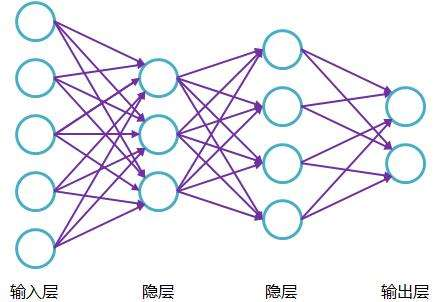
\includegraphics[width=0.7\textwidth]{figures/NN.jpg}
 \caption{多层神经网络示意图(含2个隐含层)}\label{fig:MNN}
\end{figure}

一般认为,网络结构、激活函数(activation function)和学习算法是神经网络的三大要素,神经网络的分类主要依据这三个要素。神经控制最显著的特点是具有学习能力\upcite{HanXieFu2014}。它是通过不断修正神经元之间的连接权值,并离散存储在连接网络中来实现的。它对非线性系统和难以建模的系统的控制具有良好效果。人工神经网络的模型通常可以划分为前馈神经网络和反馈神经网络等。在实际的控制系统应用中,由于反馈神经网络运算十分耗时间,因此对于在线动力学辨识和实时控制系统应用较少。前馈神经网络在解决高度非线性和严重不确定性系统的控制方面具有很大潜力。将神经网络引入控制系统是控制学科发展的必然趋势\upcite{NarendraKannan1990},出现了神经网络逆控制、神经广义预测控制、自适应神经输出反馈控制和模糊神经网络控制等方法。

对于控制界,神经网络的吸引力主要在于其强大的非线性建模与辨识能力,具体体现在以下几个方面:
\begin{enumerate}
\item 能够充分逼近任意复杂的非线性系统;
\item 能够学习和适应严重不确定系统的动态特性;
\item 由于大量神经元之间广泛连接,即使少量神经元或连接损坏,也不影响系统的整体功能,表现出很强的鲁棒性和容错性;
\item 采用并行分布处理方法,使得快速进行大量运算成为可能。
\end{enumerate}

神经网络的引入不仅给这一控制领域的突破带来了生机,也带来了许多亟待解决的问题。例如,尽管现在有很多神经控制算法,但绝大多数没有闭环系统稳定性分析;被控对象特性的不断变化和控制效果要求的不断提高使得一些传统神经控制难以达到理想的效果;快速在线学习算法是实时控制的关键,而目前大部分神经网络采用的误差反向传播(Back Propagation,BP)学习算法计算量大。因此,开发新型神经网络和快速在线学习算法并将其用于控制系统将是基于神经网络的自适应控制研究的重要方向。

\subsection{超限学习机与控制}

如前所述,目前的神经网络结构和在线学习算法难以满足控制系统的要求。传统的神经网络需要人为设置大量的网络参数;在网络训练时主要采用BP算法,需要耗费很长的时间多次迭代才能修正权值和隐元的偏置\upcite{ZhuHouXiong2005};由于使用梯度下降有陷入局部极小的缺陷,而未到达全局最小。一些研究学者也开始研究基于神经网络的实时辨识与控制算法\upcite{KorjaniBazzaz2008},但针对的是特定的问题,难以做到通用性。

2004年,黄广斌等人提出了一种新型的单隐层前馈神经网络\upcite{HuangZhuSiew2004,HangSiew2005},即超限学习机(Extreme Learning Machine, ELM)。基本的超限学习机仅需设置网络隐层节点个数,在算法执行过程中不需要调整网络的输入权值以及隐层神经元的偏置,就能产生唯一的最优解,因此具有学习速度快且泛化性能好的优点。如图\eqref{fig:elm}所示表示的是一种含有单个隐含层的多层前馈神经网络,简称为单隐层神经网络(Single-layer Neural Network , SLFN)。ELM的实现过程\upcite{HuangZhuSiew2006}主要分为三个阶段,首先初始化输入权重和隐元的偏置,然后根据输入计算出隐含层的输出,最后由期望的范数解确定输出权重,一般采用二范数,即采用最小二乘法确定。相对传统网络在保证更好的泛化性的同时具有极快的学习速度,且可以克服传统梯度算法常有的局部极小、学习时间长、性能指标及学习率等问题,朝鲜学习机表现出了对解决非线性问题极好的应用性能。

\begin{figure}
 \centering
 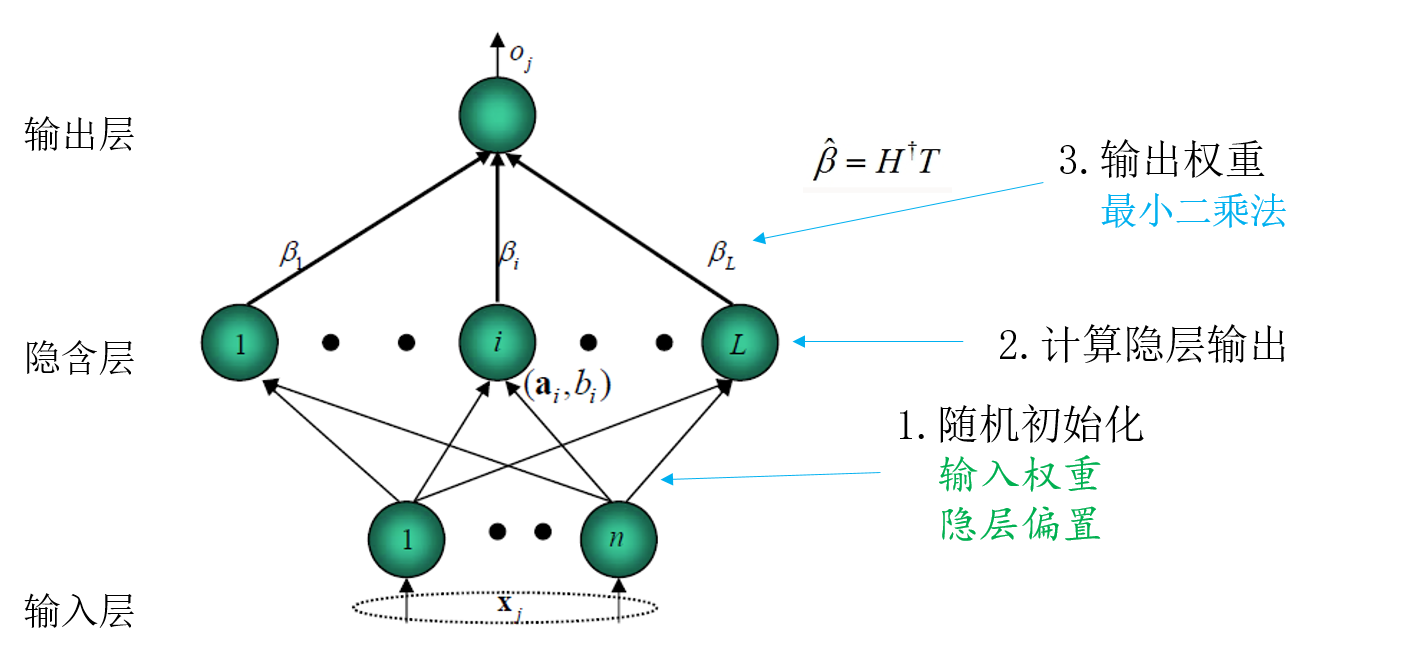
\includegraphics[width=0.7\textwidth]{figures/ELM}
 \caption{超限学习机的网络结构(单隐层)和算法流程}\label{fig:elm}
\end{figure}

超限学习机是一种简单易用、有效的前馈神经网络学习算法,在手写识别、目标跟踪等等领域\upcite{HangHang2015}取得了很大成就。它具有很好的系统辨识能力,在控制领域也出现了不少应用\upcite{RongZhao2013},特别是在线序列超限学习机(Online-sequential ELM,OS-ELM)\upcite{LiangHuang2006}及其相关变体\upcite{YangZhang2012,ShaoMeng2016},很适合解决具有强非线性的不确定性系统的辨识与控制问题\upcite{LiNai2015,WangSunMeng2016}。

\section{本文主要研究内容}

本文的主要研究对象是同时具有参数不确定性和非参数不确定性的离散时间系统,结合超限学习机对现有的半参数自适应控制进行扩展和改进。主要体现在:

本文的章节安排如下:

第一章是绪论部分,主要阐述了非线性自适应控制的研究背景和意义,总结了经典自适应控制方法的发展历程、特点与方法和存在的问题等,分析了神经网络应用于自适应估计与控制的前景和挑战,并介绍了一些新型有效的非线性辨识方法。

第二章,半参数系统与信息浓缩估计。对半参数自适应思想的来源作进一步阐述,正式描述了半参数系统的数学模型,详细介绍了信息浓缩估计的思想和具体实施方法,对原有的一阶半参数自适应估计进行了扩展。

第三章,离散时间半参数自适应控制。

第四章,连续时间半参数自适应控制。

第五章,仿真实验验证。

%%==================================================
%% chapter2.tex for BIT Master Thesis
%% version: 0.1
%% last update: Nov 8th, 2017
%%==================================================
\chapter{半参数系统与信息浓缩估计}
\label{chap:2}

传统自适应控制主要考虑系统参数不确定性,传统鲁棒控制主要考虑小范围的结构不确定性,但实际问题中参数不确定性和较大的结构不确定性可同时出现,传统方法有一定局限。半参数自适应控制给出了一种新的理论框架,解决两种不确定性同时出现的系统。现有的半参数自适应控制实现了一维情形下的参数估计算法,但二阶及其以上的参数估计并未具体实现,这涉及计算几何的知识。因此设计高阶情形下基于信息浓缩思想的参数估计算法是实现半参数自适应控制的前提。

\section{半参数系统}
\subsection{反馈机制能力与极限}

存在无法预测的不确定性,系统的输出就会产生偏差,即便是采用离散时间角度设计控制律。反馈从一开始就是为了解决这种偏差和不确定性而引入的,自适应控制从本质山说是一种非线性反馈\upcite{Guo2003}。不过当系统存在不确定性时,是否一定存在一种自适应控制律能够使得系统闭环稳定?这是在设计自适应控制之前首先要回答的问题。然而直到20世纪90年代末和本世纪初,郭雷院士等学者\upcite{XieGuo1999,ZhangGuo2002}创造性地提出反馈机制的最大能力和局限这一重要命题,同时针对类似下面表达式\eqref{eq:Guo}给出的一些基本控制系统进行定量探索,才引起来广泛的关注。
\begin{equation}%
\label{eq:Guo}
y_{k+1} = \theta f(y_{k}) + u_{k} + \omega_{k+1}
\end{equation}
其中,$u_{k}$,$y_{k}$,$\omega_{k}$ 分别是系统在$k$时刻的输入、输出和干扰,而$\theta$和$f(\cdot)$分别是待估计的参数和未知函数。系统\eqref{eq:Guo}的不确定性主要表现为函数$f(\cdot)$的未知性,这常常被称为非参数不确定性(nonparametric uncertainties);而$f(\cdot)$的绝对值随自变量$y_{k}$绝对值的增长速率决定了反馈机制能力的上限\upcite{Guo2002},在随后的研究中针对高阶情形中多元函数$f(\cdot)$,这一条件被扩展到Lipschitz条件下的规律。可以这样理解,如果$f(\cdot)$增长的比较快,那么就不存在使得系统\eqref{eq:Guo}镇定的自适应反馈控制律。分析出反馈机制的上下并给出数学证明,确实不是一件容易的事情。这一理论很直观地说明了系统的不确定性的大小常常表现为系统未知函数或者参数的变化剧烈程度,这些结论从控制稳定性和可行性的角度对系统的不确定性给出了一定的定量描述。

目前关于反馈机制及能力的研究主要针对离散时间控制系统,这与离散时间控制器的广泛应用这一大趋势不谋而合,并且一开始就考虑到了非参数不确定性,因而具有较好的理论高度和普适性。反馈机制及能力给出了对不确定性系统的认识,从理论上看,不是所有的未知系统都可以设计出稳定的自适应控制律;用但是同时也留下了一个问题:如果系统属于自适应反馈控制可稳定的范围内,那么如何设计出合适的自适应反馈控制律使系统达到满意的性能?一般来说,不同的被控对象自然结构和参数都不同,但是否存在一种较为通用的模型可以刻画大部分面对的被控对象?这样的问题可以类比经典控制理论,毕竟线性系统和微分方程这些通用工具在几十年的控制理论中起到了关键的作用。

虽然数字化控制器输出到被控对象的信号是离散时间,但是实际的过程是连续时间变化的。一般的离散时间非线性控制往往忽略了这一点,就导致这些研究侧重于理论和离散时间仿真分析。在系统\eqref{eq:NARX}中,把被控对象当成完全非线性模型,忽略了他们的线性特性,也就是说很多被控对象虽然具有较大的不确定性,但是在一定程度上是可以当作线性对象处理,只不过同时具有非线性部分,导致实际的线性部分参数与理论值有较大的偏差;对于不确定性系统,也就常常表现为同时具有参数不确定性(parametric uncertainties)和非参数不确定性。例如电机驱动系统简化处理就是一个二阶线性模型,一般的PID控制也可以获得还算不错的效果;只是在负载未知或者变化较大,以及存在一些非线性特性如库伦摩擦等情况下,会影响PID的控制效果。这一事实说明了实际系统表现出的线性特性有助于解决非线性自适应控制问题,不可忽视。这样看来,一般的非线性系统都可以看作是由线性参数部分和非线性的非参数部分组成。

\section{问题描述}
%%==================================================
%% chapter3.tex for BIT Master Thesis
%% version: 0.1
%% last update: Nov 8th, 2017
%%==================================================
\chapter{二维参数的信息浓缩估计算法}\label{chap:3}
设计高阶情形下基于信息浓缩思想的参数估计算法是实现半参数自适应控制的前提。现有的半参数自适应控制实现了一维情形下的参数估计算法,但二阶及其以上的参数估计并未具体实现,这涉及计算几何的知识。上一章介绍了半参数系统中的信息浓缩估计方法,从相关的定理\ref{thm:ic1}可知不同的先验知识会导致信息集合$I_{k}$的形式不同。一维情形由于只有一个参数不涉及顶点集的组合,因而具体算法比较容易实现,上面第\ref{subsubsect:2.3.3.1}已经给出具体计算步骤。但是实际情况往往不只有一个参数,因而需要设计多维情形的估计算法,第\ref{subsubsect:2.3.3.2}小节给出了实施框架。多维情形的算法如果直接通过代数推导,不容易解决,需要借助计算几何的思想。在线性控制理论和单变量系统中,两个参数的情况十分常见。因此本章针对两个参数即$d_{1}=2$的情形,设计信息浓缩估计器的具体算法。
\section{问题描述}\label{sect:3.1}
在第二章的基础上,本章继续考虑上下界这种典型的先验知识。如前所述,需要针对关联这种先验知识的系统设计信息浓缩估计算法,完整的过程主要以下分为两步:
\begin{enumerate}
\item 信息浓缩。在上一个时刻的基础上,根据这个时刻的输入输出数据得到的约束,确定这个时刻的信息浓缩之后的参数集合。
\item 选定合适值。根据一定的法则,从上述的参数集合中选择合适的估计值作为这个时刻的参数估计值参与控制律等后续的计算。
\end{enumerate}

第一步的具体操作是在某个确定时刻,得到一组输入输出数据,可以确定两个线性约束不等式,将这个两个约束先后加入到之前时刻的顶点集合中,得到这一时刻的顶点集合,也就确定了当前时刻的参数集合。从理论上说,第一步得到的参数集合中的每一个值都可以作为这个时刻的估计值,但是控制律等后续计算往往需要一个具体的值,所以需要按照一定的法则从集合中确定一个最优值,一般选择多边形的中心作为这个时刻的估计值。上面的两步中,第一步信息浓缩是难点。因此,本章的重点在于第一步的算法设计。一个时刻的信息浓缩过程包含两组约束关系的先后加入,也就是两次$G$变换。这两次的变换过程一样,只是每次的数据不一样,故这里只需要考虑一次变换。另外,为了叙述方便,本章关于时刻$k$的下标省略。

$d_{1}=2$时,用$\beta$和$\beta'$分别表示两个不同的多边形,其顶点集合表示(按顺时针排列,下同)为
\begin{equation*}%
\begin{split}%
\beta&=\{P_{1},P_{2},\ldots,P_{N}\}\\
\beta'&=\{P_{1}',P_{2}',\ldots,P_{N'}'\}
\end{split}
\end{equation*}

$d_{1}=2$时,关于未知参数$\bm{\theta}$的约束不等式为
\begin{equation}\label{eq.3.L}
\bm{\phi}^{T}\cdot\bm{\theta}\leq e
\end{equation}
这里$\bm{\phi}$和$\bm{\theta}$都是二维向量,$\bm{\phi}$和$e$都可以由输入输出组合得到,$\bm{\theta}$是这个不等式的未知变量。

因此,变换$G(\beta,\bm{\phi},e)$可以记为映射
\begin{equation}%
\mathbf{AddLinear2D}\colon \beta\rightarrow\beta'
\end{equation}
这就是二维参数的信息浓缩估计算法需要解决的核心部分。

\section{几何关系分析}\label{sect:3.2}
二维情形下主要是考虑同一个平面内,直线和多边形的位置关系。图\ref{fig.2d.export}展示了直线和多边形位置关系的一种可能的例子,从这个图中可以知道求解这个顶点集涉及到计算几何的知识,需要全面考虑各种情形。具体来看,分析一条直线和多边形的位置关系,就是考察多边形中每个顶点和直线的位置关系。单个顶点和直线的位置关系主要涉及平面解析几何的知识。

$d_{1}=2$时,$\bm{\phi}^{T}\cdot\bm{\theta}=e$表示一条直线$L$,它将整个平面分成两个半平面。用二元组
$$L_{c}=(\bm{\phi},\bm{\theta})$$
表示不等式约束关系
\begin{equation}\label{eq.3.neq}
\bm{\phi}^{T}\cdot\bm{\theta}\leq e
\end{equation}
在几何上,$L_{c}$也可以被认为是一个半平面。

记
$$\bm{\phi}^{T}=[\phi_{1},\phi_{2}]$$
顶点$P_{n}$的坐标为
$$P_{n}\colon (X_{P_{n}},Y_{P_{n}})$$
分别对应于待估计参数向量$\bm{\theta}$的第一个分量和第二个分量。

顶点$P_{n}$和直线$L$的位置关系可以由下面的不等式确定
\begin{equation}\label{eq.3.L.P}
\phi_{1}X_{P_{n}}+\phi_{2}Y_{P_{n}}\leq e
\end{equation}

如果不等式\eqref{eq.3.L.P}成立,则顶点$P_{n}$满足约束关系\eqref{eq.3.neq},即在半平面$L_{c}$内;否则,顶点$P_{n}$不在半平面$L_{c}$内。根据不等式\eqref{eq.3.L.P}可以确定多边形$\beta$的所有顶点和直线$L$的位置关系,从而判断出这个多边形和直线的位置关系。

经过分析,根据各个顶点和直线的分布情况,可以将多边形和直线的位置关系分为三类。
\begin{enumerate}
\item 多边形顶点在直线的同一侧,则多边形和直线没有交点,如图\ref{fig.3.beta.l.1}所示又可具体分为两种情况。第一种情况\ref{fig.poly.1.1},多边形不变,即$\beta'=\beta$;第二种情况\ref{fig.poly.1.2},一般是在数据出错的情况下才会发生(在定理\eqref{thm:ic1}已经指出),此时$\beta'=\varnothing$,算法停止。
\begin{figure}[htp]
	\centering
	\subfigure[情形1.1]{	 % Caption of subfigure in []
	\label{fig.poly.1.1}	 % Label of subfigure in {}
	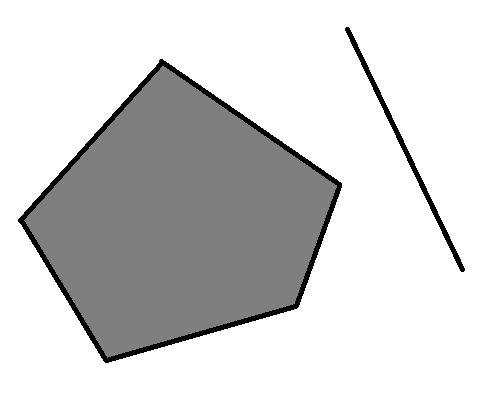
\includegraphics[width=0.4\textwidth ]{ch3-poly-00.png}}
	\subfigure[情形1.2]{
	\label{fig.poly.1.2}
	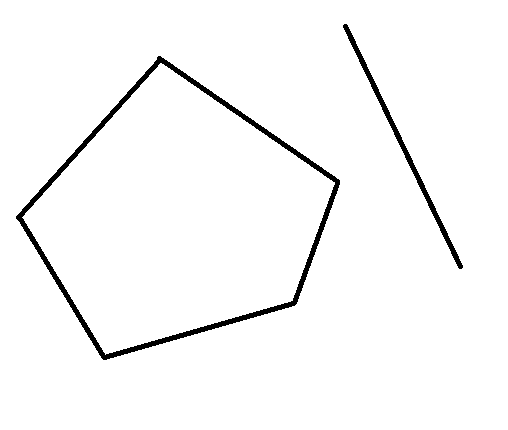
\includegraphics[width=0.4\textwidth ]{ch3-poly-01.png}}
	\caption{直线和多边形位置关系的第一类情形}	 % Caption of figure
	\label{fig.3.beta.l.1}	 % Label of figure
\end{figure}
\item 多边形只有一个顶点和其他顶点不在直线的同一侧,如图\ref{fig.3.beta.l.2}所示又可具体分为两种情况。第一种情况\ref{fig.poly.2.1},只有一个顶点不满足约束,多边形顶点个数加1;第二种情况\ref{fig.poly.2.2},只有一个顶点满足约束,多边形变成一个三角形。
\begin{figure}[htp]
	\centering
	\subfigure[情形2.1]{	 % Caption of subfigure in []
	\label{fig.poly.2.1}	 % Label of subfigure in {}
	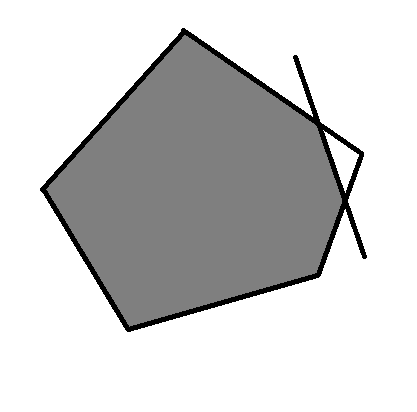
\includegraphics[width=0.4\textwidth ]{ch3-poly-10.png}}
	\subfigure[情形2.2]{
	\label{fig.poly.2.2}
	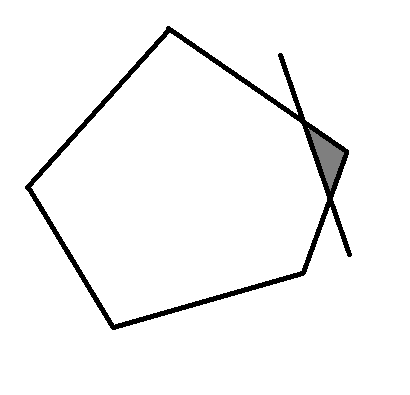
\includegraphics[width=0.4\textwidth ]{ch3-poly-11.png}}
	\caption{直线和多边形位置关系的第二类情形}	 % Caption of figure
	\label{fig.3.beta.l.2}	 % Label of figure
\end{figure}
\item 多边形有至少两个顶点和其他顶点不在直线的同一侧,如图\ref{fig.3.beta.l.2}所示又可具体分为两种情况。图\ref{fig.poly.3.1}和\ref{fig.poly.3.2}是两种对立的情形,事先都无法准确知道剩余的顶点个数,只能根据实际情况确定。
\begin{figure}[htp]
	\centering
	\subfigure[情形3.1]{	 % Caption of subfigure in []
	\label{fig.poly.3.1}	 % Label of subfigure in {}
	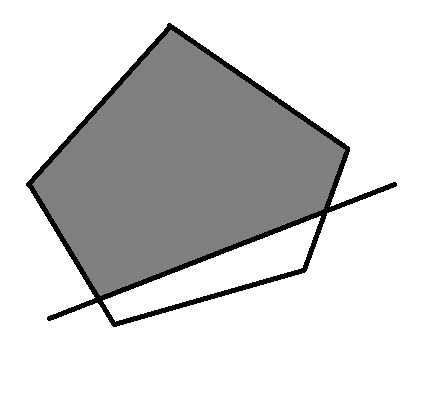
\includegraphics[width=0.4\textwidth ]{ch3-poly-20.png}}
	\subfigure[情形3.2]{
	\label{fig.poly.3.2}
	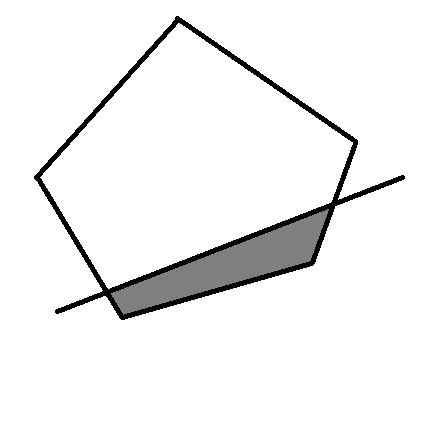
\includegraphics[width=0.4\textwidth ]{ch3-poly-21.png}}
	\caption{直线和多边形位置关系的第三类情形}	 % Caption of figure
	\label{fig.3.beta.l.3}	 % Label of figure
\end{figure}
\end{enumerate}

\section{算法实现}\label{sect:3.3}
根据上节关于多边形和直线的几何位置关系的分析和总结,本节设计了$d_{1}=2$时多边形顶点集变换$\mathbf{AddLinear2D}$的计算几何算法。

需要遍历多边形的所有顶点与多边形的位置关系。可以用一个数组记录顶点$P_{n}$和约束$L_{c}$的位置关系,即
\begin{equation}%
\mathbf{Flag}(n)=\left\{
\begin{aligned}%
&1,\ P_{n}\in L_{c}\\
&-1,\ P_{n}\in L_{c}
\end{aligned}
\end{equation}
这里,$n=1,2,\ldots,N$。

根据上节的位置关系结果,可以设计算法的流程图如图\ref{fig.3.ic.flow}所示。
\begin{figure}[htb]
 \centering
 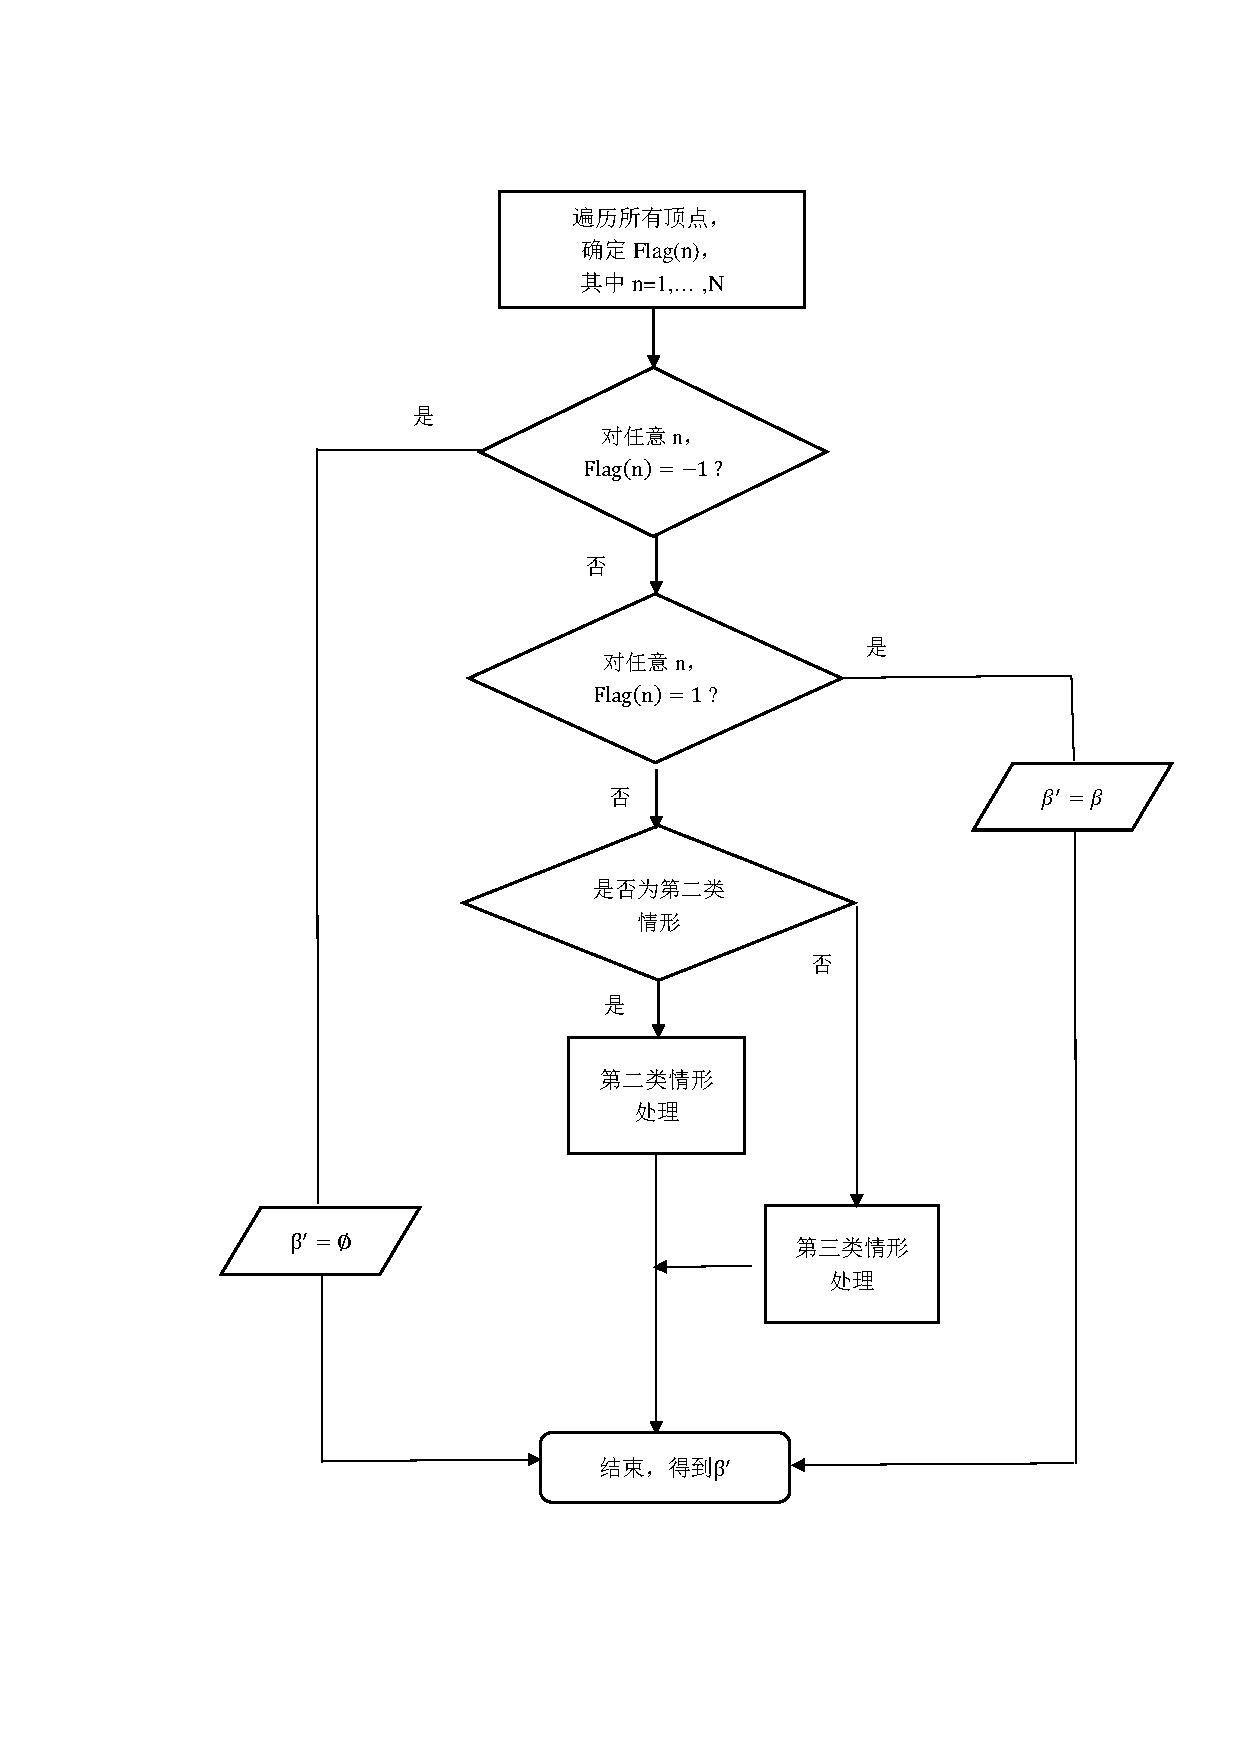
\includegraphics[width=0.9\textwidth ]{ch3-lc-flow.pdf}\\	 % e.g.,[scale=0.75], [width=0.75\textwidth ]
 \caption{$\mathbf{AddLinear2D}$的算法流程图}
 \label{fig.3.ic.flow}
\end{figure}

最后写出具体过程伪代码实现见算法\ref{alg.ic.2d}。
\begin{algo}%
\caption{$\mathbf{AddLinear2D}$}
\label{alg.ic.2d}
\begin{algorithmic}
\REQUIRE $\beta=\{P_{1},P_{2},\ldots,P_{N}\}$\\
\ENSURE $\beta'=\{P_{1}',P_{2}',\ldots,P_{N'}'\}$\\
\STATE Denote the number of vertices in $\beta$ by $N$
\FOR{$j=1$ to $N$}
	\STATE Denote the $jth$ vertex by $P_{j}$
	\STATE Let $F_{j}=\mathbf{sgn}(c-\phi^{T}P_{j})$
\ENDFOR
\IF{$F_{j}\geq0\ \forall 1\leq j\leq n$}
	\STATE $\beta'\leftarrow\beta$ and return
\ELSIF{$F_{j}<0\ \forall 1\leq j\leq n$}
	\STATE $\beta\leftarrow\emptyset$ and return
\ENDIF
\FOR{$j=2$ to $N-1$}
    \IF{($P_{j}$ and $P_{j-1}$ are in different sides) $\bigwedge$ ($P_{j}$ and $P_{j+1}$ are in different sides)}
		\STATE $P_{1}^{i}\leftarrow$ the intersection of $l_{i}$ and $\overline{P_{j-1}P_{j}}$
		\STATE $P_{2}^{i}\leftarrow$ the intersection of $l_{i}$ and $\overline{P_{j+1}P_{j}}$.
		\IF {($F_{j}>0$)}
			\STATE$\beta'=\{P_{1}^{i},P_{j},P_{2}^{i}\}$
		\ELSE
			\STATE$\beta'=\{P_{1},\ldots,P_{j-1},P_{1}^{i},P_{2}^{i},P_{j+1},\ldots,P_{n}\}$
		\ENDIF
        \STATE break
    \ELSIF{($P_{j},P_{j-1}$ are in different sides) $\bigwedge$ ($P_{j},P_{j+1},\ldots,P_{j+a-1}$ are on the same side) $\bigwedge$ 
		($P_{j+a-1},P_{j+a}$ are on different sides)}
		\STATE $P_{1}^{i}\leftarrow$ the intersection of $l_{i}$ and $\overline{P_{j-1}P_{j}}$
		\STATE $P_{2}^{i}\leftarrow$ the intersection of $l_{i}$ and $\overline{P_{j+a-1}P_{j+a}}$.
		\IF {($F_{j}>0$)}
			\STATE$\beta'=\{P_{1}^{i},P_{j},\ldots,P_{j+a-1},P_{2}^{i}\}$
		\ELSE
			\STATE$\beta'=\{P_{1},\ldots,P_{j-1},P_{1}^{i},P_{2}^{i},P_{j+a},\ldots,P_{n}\}$
		\ENDIF
        \STATE break
	\ELSIF{($P_{j},P_{j+1}$ are in different sides) $\bigwedge$ ($P_{j},P_{j-1},\ldots,P_{j-b+1}$ are on the same side) $\bigwedge$ 
	($P_{j-b+1},P_{j-b}$ are on different sides)}
		\STATE $P_{1}^{i}\leftarrow$ the intersection of $l_{i}$ and $\overline{P_{j-b+1}P_{j-b}}$
		\STATE $P_{2}^{i}\leftarrow$ the intersection of $l_{i}$ and $\overline{P_{j+1}P_{j}}$.
		\IF {($F_{j}>0$)}
			\STATE$\beta'=\{P_{1}^{i},P_{j-b+1},\ldots,P_{j},P_{2}^{i}\}$
		\ELSE
			\STATE$\beta'=\{P_{1},\ldots,P_{j-b},P_{1}^{i},P_{2}^{i},P_{j+1},\ldots,P_{n}\}$
		\ENDIF
        \STATE break
    \ENDIF
	\STATE $j\leftarrow j+1$
\ENDFOR
\STATE return $\beta'$
\end{algorithmic}
\end{algo}

算法\ref{alg.ic.2d}实现了第\ref{sect:3.1}中提到的信息浓缩估计的第一步。对于第二步,一般选择多边形$\beta'$的中心作为参数估计值$\hat{\bm{\theta}}$,即
\begin{equation}\label{eq.3.theta}
\begin{split}%
&\hat{\theta}_{1}=\frac1N\sum_{n=1}^{N}X_{P'_{n}}\\
&\hat{\theta}_{2}=\frac1N\sum_{n=1}^{N}Y_{P'_{n}}
\end{split}
\end{equation}

本节设计的算法\ref{alg.ic.2d}和方程\eqref{eq.3.theta}就是$d_{1}=2$时完整的信息浓缩估计算法,可以用于后续的控制器设计。

\section{仿真实例}\label{sect:3.4}
为了验证本章设计算法的有效性,本节在实际的被控对象中仿真上面设计的信息浓缩估计算法。选择如下的被控对象
\begin{equation}
\label{eq.3.sys.eq}
y_{k+1}=\theta_{1}\cdot y_{k} +\theta_{2}\cdot y_{k-1}+u_{k}+\omega_{k+1}+\sin(\frac{k}2)
\end{equation}
其中$\theta_{1}=-0.5$,$\theta_{2}=0.5$。随机干扰取为均匀分布,即
\begin{equation*}
\omega_{k}\in U(0,1) 
\end{equation*}
则随机干扰的上下确界为
\begin{equation*}
0\leq\omega_{k}\leq1
\end{equation*}
而非线性部分是三角函数,其上下界为
\begin{equation*}
-1\leq\sin(\frac{k}2)\leq1
\end{equation*}

为了便于计算,令$u_{k}=0$。在本节中,为了更加符合实际情况,在计算时,将随机干扰和非线性的上下界范围扩大,分别取为
\begin{equation*}
-1\leq\omega_{k}\leq2
\end{equation*}
和
\begin{equation*}
-2\leq\sin(\frac{k}2)\leq2
\end{equation*}
因此,合并得到
\begin{equation*}
\begin{split}%
&\underline{z}=-3\\
&\overline{z}=4
\end{split}
\end{equation*}

初始的参数集合取为
\begin{equation*}%
\Theta=\{-1\leq\theta_{1}\leq1,\ -1\leq\theta_{2}\leq1\}
\end{equation*}

仿真到第$k=500$时,得到的多边形如图\ref{fig.3.poly}所示,其中红色圈点代表真实值$\bm{\theta}$在几何上的表示,星形点代表了估计值$\hat{\bm{\theta}}$在几何上的表示。画出整个仿真过程的参数估计曲线如图\ref{fig.3.theta.hat}所示。从这个图中可以看出,参数估计值接近真实值。
\begin{figure}[!h]
	\centering
	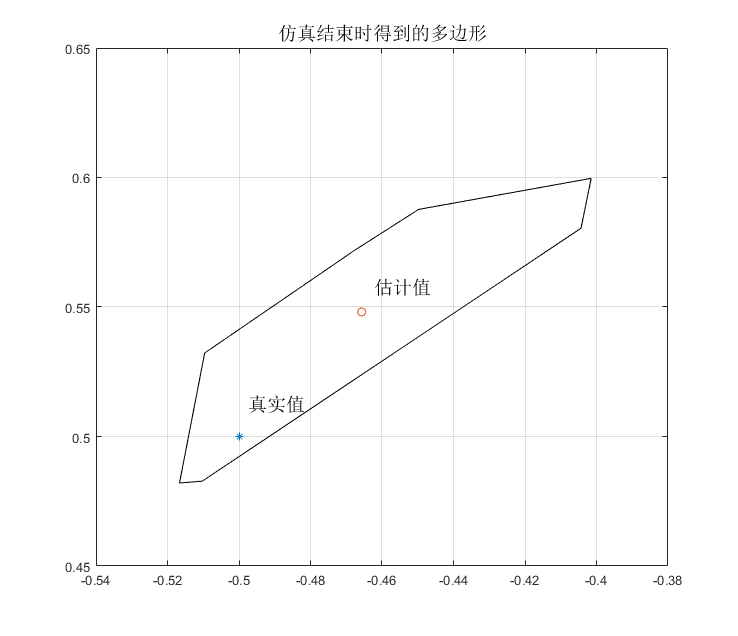
\includegraphics[width=0.7\textwidth ]{ch3-2d-poly.png}\\	 % e.g.,[scale=0.75], [width=0.75\textwidth ]
	\caption{当$d_{1}=2$时仿真实例中$k=500$时的多边形及参数估计}
	\label{fig.3.poly}
\end{figure}

\begin{figure}[h]
	\centering
	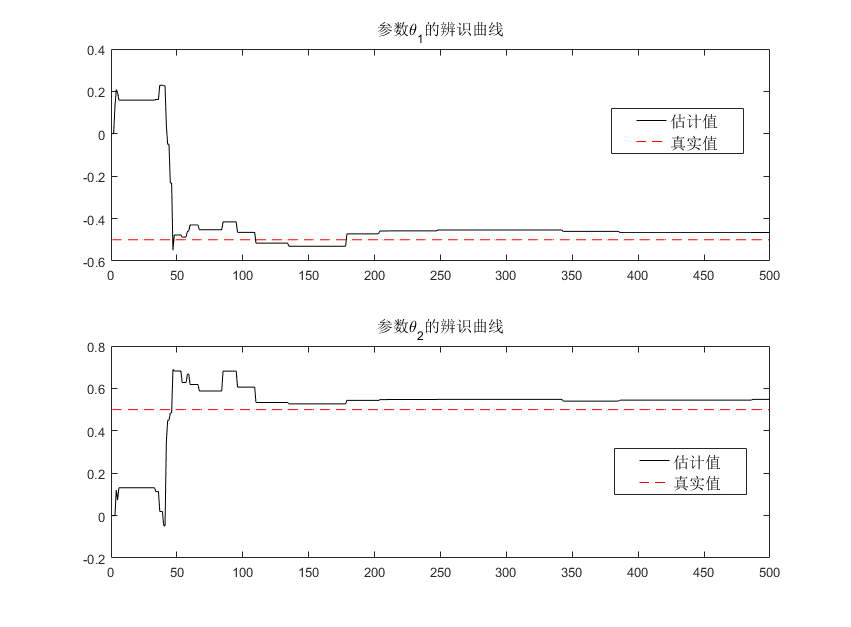
\includegraphics[width=0.8\textwidth ]{ch3-2d-theta.png}\\	 % e.g.,[scale=0.75], [width=0.75\textwidth ]
	\caption{当$d_{1}=2$时仿真实例中的参数估计曲线(信息浓缩估计算法)}
	\label{fig.3.theta.hat}
\end{figure}

\section{优化问题}\label{sect:3.5}
在信息浓缩估计方法中,关键的问题在于计算每一步(时刻$k$)的信息集$I_{k}$和信息浓缩集$C_{k}$。从上面的讨论中,可以看出$d_{1}=1$时很容易解决这两个集合的计算问题。然而,当$d_{1}>1$时,通常情况下集合$C_{k}$中的顶点个数$N_{k}$随着$k\rightarrow\infty$会不断增长,特别是高维情形$d_{1}\geq3$时。因此,有可能在实际应用中,随着$k\rightarrow\infty$,信息浓缩估计过程需要的内存会无限增长,这是一个十分致命的问题,需要优化。

其实,随着$k\rightarrow\infty$,$C_{k}$的范围是在不断缩小的,即使顶点个数可能会增加。因此,为了克服顶点个数无限增长的问题,在实际应用中,可以不需要如此多的顶点来精确的表示信息浓缩集$C_{k}$。也就是说,在多维情形中,在每个时刻$k$的$G$变换过程中,可以用具有足够少顶点个数$N_{L}$的集合$\hat{C}_{k}$来近似$C_{k}$。

一般有两种优化策略,这里主要介绍被称为信息浓缩估计算法的“松实现”(Loose IC estimator, Loose-IC),另外一种是“紧实现”(Tight IC estimator, Tight-IC)。Loose-IC的具体要求是,对于任意的$k$,都满足$\hat{C}_k\supseteq C_k$.

记$$\hat{C}_{\infty}=\bigcap\limits_{k=1}^{\infty} \hat{C}_{k},$$
则
\begin{equation}\label{eq.loose}
C_{\infty}=\bigcap\limits_{k=1}^{\infty} C_{k}\subseteq \hat{C}_{\infty}
\end{equation}

上面方程\eqref{eq.loose}意味着,Loose-IC在实施过程中不会丢弃任何可能的参数值。对于$d_{1}=2$这种二维情形,为了便于计算,一般选择顶点个数$N_{L}=3$或者$N_{L}=4$,分别如图\ref{fig.3.loose.3}和\ref{fig.3.loose.4}所示。从图中可以看出,顶点个数的减少和多边形的简化,意味者计算复杂度的降低,实现较好的优化效果。
\begin{figure}[h]
 \centering
 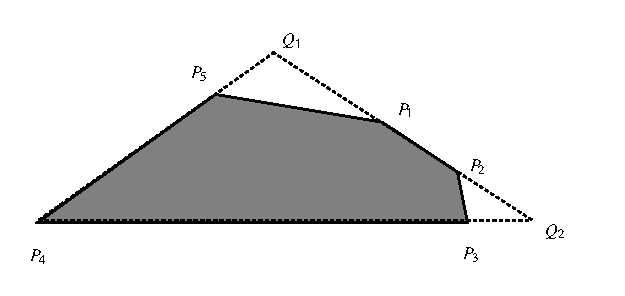
\includegraphics[width=0.7\textwidth ]{fig-loose-export.eps}\\	 % e.g.,[scale=0.75], [width=0.75\textwidth ]
 \caption{$d_{1}=2$且$N_{L}=3$时的Loose-IC实现,用三角形近似多边形}
 \label{fig.3.loose.3}
\end{figure}
\begin{figure}[h]
 \centering
 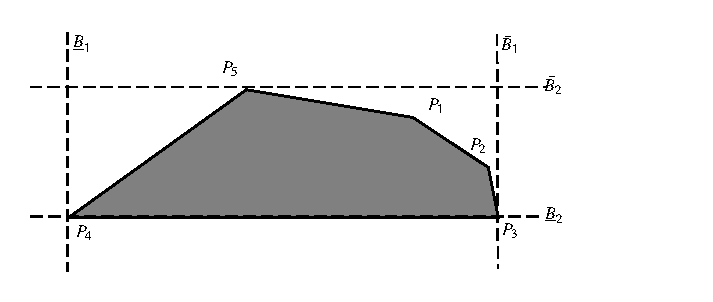
\includegraphics[width=0.7\textwidth ]{fig-rect-export.eps}\\	 % e.g.,[scale=0.75], [width=0.75\textwidth ]
 \caption{$d_{1}=2$且$N_{L}=4$时的Loose-IC实现,用矩形近似多边形}
 \label{fig.3.loose.4}
\end{figure}

\section{主要特点}\label{sect:3.6}
从上面的讨论和仿真实例中,可以总结出信息浓缩估计算法有如下优点:
\begin{enumerate}
\item 充分利用先验信息和后验数据产生的信息。理想情况下没有任何的信息被浪费掉,而一般传统的辨识算法仅仅利用了部分先验信息和某些随机先验假设。
\item 这是基于集合的估计,实际上每次给出的是一个参数可行的集合,不同于最小二乘算法等给出的点估计,即单个值。这样一方面可以获得比较全面的参数信息,另一方面可以衡量估计值的准确性。
\item 随着时间的增长,逐步找出最优(最有可能的)参数估计值。在参数估计过程中,同时可以用于检查实际采集的数据和系统模型的先验信息的一致性。
\item 可以针对随机系统,也可以处理非统计语言描述的先验信息,不受限于概率模型。
\item 具体实施比较灵活,主要取决于先验信息的具体表现形式,这也给算法的优化带来了极大的提升空间。例如为了降低计算复杂度,可以用上节讨论的“松实现”。
\item 不像传统辨识算法一样,在某些时候表现出随着时间的推移,估计值漂移或者精度下降的现象。相反,数据越多,估计越准确。
\end{enumerate}
一般事物总存在两面性,经过分析,信息浓缩估计算法也存在如下问题:
\begin{enumerate}
\item 难以利用系统干扰项的先验信息,特别是无界随机干扰。也许在这种没有非参数不确定性且随机干扰是无界噪声序列时,传统基于值估计的算法表现得更加适合。
\item 实际的算法效率依赖于先验信息的利用程度和具体实现。一般情况下,由于信息浓缩估计算法涉及到计算几何过程(也许有其他的实施策略),因而其计算复杂度和设计难度要稍大于RLS等传统辨识算法。毕竟后者一般只会涉及到矩阵的加减乘除运算。
\item 目前不存在针对信息浓缩估计算法的显示表达式或者固定的公式,同时,基于集合的辨识思路给具体控制系统的应用和闭环稳定性分析带来了一定的困难。
\end{enumerate}

虽然存在诸如此类的缺点,但信息浓缩估计算法仍然提供了很好的辨识思路和较好的收敛性和精确度,值得深入研究和进一步优化。

\section{本章总结}
本章主要讨论了信息浓缩估计算法的具体实现。首先描述了二维参数情形下,信息浓缩估计算法的主要步骤和基本问题;然后对信息浓缩变换中直线和多边形的几何关系进行了详细地分析,同时设计了信息浓缩变换的算法流程图,并给出了具体的伪代码实现;接着在实际的被控对象中仿真前面设计的信息浓缩估计算法,给出了最终估计结果和过程曲线;最后讨论了信息浓缩估计的计算复杂度优化问题,总结了信息浓缩估计的主要优缺点。
%%==================================================
%% chapter4.tex for BIT Master Thesis
%% version: 0.1
%% last update: Nov 8th, 2017
%%==================================================
\chapter{离散时间半参数自适应控制}\label{chap:4}
自适应控制中的辨识是为了最终解决控制问题。上一章设计了二维情形下的信息浓缩估计算法去辨识线性部分的未知参数。本章将在第三章的基础上,利用一种机器学习算法设计非参数部分的估计方法,然后根据两部分不确定性的估计结果设计自适应控制律,解决随动控制问题。

\section{问题描述}\label{sect:4.1}
半参数系统建模方法可以适用于很多复杂的系统,但是直接研究多输入多输出等复杂模型不利于设计控制算法,而往往从简单的模型出发更能深入理解实际系统的本质。再次考虑第二章给出的半参数模型
\begin{equation}%
\label{eq:4.semi-u}
y_{k+1} = \bm{\theta}^{\tau}\bm{\phi_{k}}+u_{k}+f(\bm{\bm{\psi}_{k}})+\epsilon_{k+1}
\end{equation}
其中,$\bm{\theta}$是未知参数向量,$f(\cdot)$是未知函数。令
\begin{equation}
z_{k} = f(\bm{\psi}_{k}) + \epsilon_{k+1}
\end{equation}

针对系统\eqref{eq:4.semi-u},自适应估计与控制问题的一般表述:给定关于$\bm{\theta}$,$f(\cdot)$和$\epsilon_{k+1}$的先验信息,在$k$时刻,如何根据实时产生的一系列输入输出数据$\{y_{k},u_{k};k=1,2,\ldots\}$,去估计未知参数$\bm{\theta}$和$z_{k}$?然后根据$\bm{\theta}$和$z_{k}$的估计(预测)值去设计合适的自适应控制输入$u_{k}$使得$k+1$时刻的输出$y_{k+1}$能跟踪上期望的输出$y_{k+1}^{*}$。

本章针对系统\eqref{eq:4.semi-u}有如下先验信息:
\begin{itemize}
\item 期望跟踪信号$\{y_{k}^{*}\}$是有界的,即存在有界正常数$B_{yd}$,使得
\begin{equation}\label{eq:4.ydB}
|y_{k}^{*}|\leq B_{yd},\ \forall k\geq0.
\end{equation}
\item $\bm{\theta}$各分量是有界的,即$\underline{\theta}_{j}\leq\theta_{j}\leq\overline{\theta}_{j}$,其中$\underline{\theta}_{j}$和$\overline{\theta}_{j}$为已知的常数,$j=1,2,\ldots,d_{1}$.
\item 噪声序列$\epsilon_{k}$的取值在一个已知的范围内,即
\begin{equation}\label{eq:4.wB}
\underline{\epsilon}\leq\epsilon_{k}\leq\overline{\epsilon},\ \forall k\geq0.
\end{equation}
\item 未知函数$f(\cdot)$的上下界受限于其他已知函数,即
\begin{equation}\label{eq:4.fB}
\underline{f}(\bm{\psi})\leq f(\bm{\psi})\leq \overline{f}(\bm{\psi}).
\end{equation}
\end{itemize}

第三章已经给出了$\bm{\theta}$的估计算法,因此剩下的部分可以分为两个核心问题,一方面是设计$f(\cdot)$的估计算法,另一方面是设计控制输入$u_{k}$的表达式。假设第二章设计出的未知参数的估计值为$\hat{\bm{\theta}}_{k}$,下面需要设计出$\breve{z}_{k}$的表达式。因此,根据必然等价原理,设计出的控制输入的一般表达式为:
\begin{equation}\label{eq:4.uk}
u_{k}^{*}=y_{k+1}^{*}-\bm{\phi_{k}}^{\tau}\hat{\bm{\theta}}_{k}-\breve{z}_{k}
\end{equation}
非线性部分的辨识与控制器的设计是本章要重点解决的问题。

\section{非参数部分的估计}\label{sect:4.2}
\subsection{最近邻估计}
前面的章节用信息浓缩估计解决了参数不确定性的辨识问题,现有的半参数自适应控制方法针对非参数部分使用的是最近邻估计,其针对的主要是一维参数情形($d_{1}=1$且$d_{2}=1$),即下面的一维半参数系统
\begin{equation}%
\label{eq:4.1ord}
y_{k+1}=\theta y_{k}+u_{k}+f(y_{k})+\epsilon_{k+1}
\end{equation}
这里,标量$\theta$是未知的,为系统的参数不确定性部分,同样$f(\cdot)$是非参数不确定性部分,满足Lipschitz条件。最近邻估计不直接地估计$f(\cdot)$部分,而是直接估计
\begin{equation}\label{eq:4.nne.g}
\eta_{k} = \theta y_{k}+f(y_{k})
\end{equation}
这个整体。这样,在用信息浓缩算法估计出参数$\theta$之后,移除这个估计值$\hat{\theta}$,就可以获得非参数部分的估计。

在系统\eqref{eq:4.1ord}中,由于Lipschitz条件的存在,不管是非参数部分还是参数部分都主要和输出值$y_{k}$相关,这样输出值$y_{k}$相近的时刻,那么$\eta_{k}$的值也应该相差不大。因此最近邻估计就主要利用到了这一点,其主要思想在于寻找和当前时刻输出值$y_{k}$最相近的时刻,然后进行比较计算。

首先定义最近邻时刻为
\begin{equation}\label{eq:4.it}
i_k\triangleq\mathop{\arg \min}\limits_{i<k}|y_k-y_i|
\end{equation}
$i_k$是历史输出值中和当前时刻最接近的时刻。那么有如下等式成立
\begin{equation*}
\begin{array}{lll}
&\eta_k&=\eta_k-z_{i_k}+z_{i_k}\\
&&=[\theta y_k+f(y_k)]-[\theta y_{i_k}+f(y_{i_k})+w_{i_k+1}]+z_{i_k}\\
&&=[\theta(y_k-y_{i_k})+z_{i_k}]+[f(y_k)-f(y_{i_k})-w_{i_k+1}]
\end{array}
\end{equation*}
一般来说,上面等式中的最后一行中$f(y_k)-f(y_{i_k})$的值接近零,并且干扰项比较小。因此,可以取整体表达式\eqref{eq:4.nne.g}的估计为
\begin{equation}\label{eq.4:g.est}
\begin{array}{lll}
\hat{\eta}_k&\triangleq\hat{\theta}_k(y_t-y_{i_k})+z_{i_k}
&=\hat{\theta}_{k}(y_k-y_{i_k})+(y_{i_k+1}-u_{i_k})
\end{array}
\end{equation}
接着,令
\begin{equation}\label{eq.4:bk}
\begin{array}{lll}
\bar{b}_k\triangleq \max\limits_{i\leq k}y_i
         =\max(\bar{b}_{k-1}, y_k)\\
\underline{b}_k\triangleq \min\limits_{i\leq k}{y_i}
                =\min(\underline{b}_{k-1}, y_k).
\end{array} 
\end{equation}
最后基于最近邻估计思想设计出下面的控制律
\begin{equation}\label{eq:4.uk}
u_{k}=\left\{
\begin{array}{cc}
  -\hat \eta_k+y_{k+1}^* & \text{if } |y_k-y_{i_k}|\le D \\
  -\hat \eta_k+\frac12(\bar b_k+\underline b_k) & \text{if } |y_k-y_{i_k}|> D \\
\end{array}
\right.
\end{equation}
这里,$D$是一个合适的常数值。

由此看出,最近邻估计可以比较准确地给出一维情形下非参数部分的估计,从而解决半参数系统的自适应控制问题。但是有一定的局限性,主要体现在如下:
\begin{enumerate}
\item 由于最近邻时刻$i_k$的计算需要遍历所有的历史值,因此,随着时间的增长,理论上需要无限的内存用来存储历史数据。这给实施带来了困难。
\item 由于在计算$\hat{g}_k$时没有对干扰值作特别处理,因此适用于干扰值的有界范围比较小且变化比较慢的系统。
\item 没有充分利用历史数据和关联先验信息,只是利用最近邻时刻的数据,计算结果不一定是最优的。
\end{enumerate}

以上的缺点存在,导致现有的半参数自适应控制存在很大的局限性。本章借助于其他的非线性辨识算法去设计新的非参数部分的估计算法。

\subsection{神经网络}
机器学习解决的问题从数学上主要分为分类和回归。其中分类处理的数据主要是离散型数据,回归解决的对象和思路跟控制中的估计、预测十分类似。而神经网络作为一种十分有效的回归与预测算法,在非线性辨识中应用十分广泛。神经网络主要由输入层、隐含层和输出层组成(最简单的神经网络可能没有隐含层),依据不同的激活函数或者不同的学习算法,种类十分丰富。

本章以及本文主要讨论一种十分常见的单隐层前馈神经网络(Single hidden layer feedforwar network, SLFN),即具有一个输入层、一个隐含层以及一个输出层的前馈型神经网络。这是一种多层神经网络,其中位于输入层的神经元接受外界输入,隐含层与输出层的神经元按照一定规则对数据进行处理,整个网络的最终结果由位于输出层的神经元输出。

下面首先阐述神经网络的基本数学模型。对于一个具有$N_{i}$个输入神经元、$N_{o}$个输出神经元以及$N_{h}$个隐含层神经元的单隐层前馈神经网络来说,如果其激活函数为$g(\cdot)$,并存在$N_{s}$个输入输出样本对
$$\{\bm{x}_{j},\bm{t}_{j}\},\ j=1,2,\ldots,N_{s}$$
这里,输入向量为
$$\bm{x}_{j}=[x_{j,1},x_{j,2},\ldots,x_{j,N_{i}}]^{\tau}\in \mathcal{R}^{N_{i}}$$
期望的输出向量为
$$\bm{t}_{j}=[t_{j,1},t_{j,2},\ldots,t_{j,N_{o}}]^{\tau}\in \mathcal{R}^{N_{o}}$$
则对于任意输入向量$\bm{x}_{j}$,第$l$个($l=1,2,\dots,N_{o}$)输出层神经元的输出为
\begin{equation}%
\label{eq:4.slfn.o}
\begin{split}%
o_{j,l}&=\sum_{i=1}^{N_{h}} \beta_{i,l} g(\bm{w}_{i},b_{i},\bm{x}_{j})\\
&=\sum_{i=1}^{N_{h}} \beta_{i,l} h(\bm{x}_{i})\\
&=\bm{h}(\bm{x}_{j})^{\tau}\cdot\bm{\beta}_{l}
\end{split}
\end{equation}
其中,$\bm{w}_{i}$和$b_{i}$分别是连接第$i$个隐层神经元与输入层的权重向量和阈值,$\bm{\beta}_{l}$是连接隐含层和第$l$个输出层神经元的权重向量,$\bm{h}(\bm{x}_{j})$为隐含层的输出向量。

一般来说,同一层的激活函数是一致的。如果第$i$个隐含神经元的激活函数$g(\cdot)$是加性的(addictive),比如Sigmoid型或者正弦型,则其输出为
\begin{equation}%
g(\bm{w}_{i},b_{i},\bm{x}_{j})=g(\bm{w}_{i}^{\tau}\cdot\bm{x}_{j}+b_{i})
\end{equation}
如果是径向基(Radias base function, RBF)网络,则
\begin{equation}%
g(\bm{w}_{i},b_{i},\bm{x}_{j})=g(b_{i}\|\bm{x}_{j}-\bm{w}_{i}\|)
\end{equation}
此时,$g$是某种径向对称的标量函数,通常定义为关于样本到数据中心$\bm{w}_{i}$之间的欧氏距离的单调函数,比如高斯径向基函数等。在RBF网络的命名上,$\bm{w}_{i}$和$b_{i}$一般不称为隐层的权重和阈值,而是激活函数的中心(center)和影响因子(impact factor)。

理论上,对于给定的样本数据集,上述定义的具有$N_{h}$个隐含层神经元和激活函数为$g(\cdot)$的SLFN,具有近似零误差地逼近$N_{s}$个样本的性质\upcite{ZhouML2016},即
\begin{equation*}
\sum_{j=1}^{N_{h}}\|o_{j}-t_{j}\|=0,\ j=1,2,\dots,N_{s}
\end{equation*}
这意味着,存在一组$\bm{w}_{i}$、$b_{i}$和$\bm{\beta}$,使得
\begin{equation}
\bm{h}(\bm{x}_{j})^{\tau}\bm{\beta}=t_{j},\ j=1,2,\dots,N_{s}
\end{equation}
将上面$N_{s}$个方程堆积起来,写成紧凑的矩阵形式就是
\begin{equation}\label{eq:4.nn.HT}
\bm{H}\bm{\beta}=\bm{T}
\end{equation}
其中,$\bm{H}$是隐含层的输出矩阵,具体为
\begin{equation}\label{eq:4.nn.H}
\begin{split}
&\bm{H}(\bm{w}_{1},\cdots,\bm{w}_{N_{h}};b_{1},\cdots,b_{N_{h}};\bm{x}_{1},\cdots,\bm{x}_{N_{s}})=\\
&\begin{bmatrix}
&h(\bm{w}_{1},b_{1},\bm{x}_{1}) &\cdots &h(\bm{w}_{N_{b}},b_{N_{h}},\bm{x}_{N_{1}})\\
&\vdots &\ddots & \vdots\\
&h(\bm{w}_{1},b_{1},\bm{x}_{N_{s}}) &\cdots &h(\bm{w}_{N_{b}},b_{N_{h}},\bm{x}_{N_{s}})
\end{bmatrix}_{N_{s}\times N_{h}}
\end{split}
\end{equation}
\begin{equation}\label{eq:4.nn.beta}
\bm{\beta} = \begin{bmatrix}%
&\bm{\beta}_{1}^{\tau}\\
&\vdots\\
&\bm{\beta}_{N_{h}}^{\tau}
\end{bmatrix}_{N_{h}\times N_{o}}
\end{equation}
且
\begin{equation}\label{eq:4.nn.T}
\bm{T} = \begin{bmatrix}%
&\bm{t}_{1}^{\tau}\\
&\vdots\\
&\bm{t}_{N_{h}}^{\tau}
\end{bmatrix}_{N_{s}\times N_{o}}
\end{equation}

如果隐含层神经元个数等于样本的个数,即$N_{s}=N_{h}$,那么矩阵$\bm{H}$是方阵且可逆的,则SLFN可以实现零误差逼近的结果。然而,在实际的大多数情况下,隐含层神经元个数远小于样本个数,即$N_{h}\ll N_{s}$。这样,$\bm{H}$不是一个方阵,就不存在准确的一组$\bm{w}_{i}$、$b_{i}$和$\bm{\beta}$,使得$\bm{H}\bm{\beta}=\bm{T}$精确成立。这种情况下,神经网络学习的目标就是寻找合适的一组$\hat{\bm{w}}_{i}$、$\hat{b}_{i}$和$\hat{\beta}$,使得
\begin{equation}\label{eq:4.nn.H-T}
\begin{split}%
&\|\bm{H}(\hat{\bm{w}}_{1},\dots,\hat{\bm{w}}_{N_{h}};\hat{b}_{1},\dots,\hat{b}_{N_{h}})\hat{\bm{\beta}}-\bm{T}\|=\\
&\min_{\hat{\bm{w}}_{i},\hat{b}_{i},\hat{\bm{\beta}}}\|\bm{H}(\bm{w}_{1},\dots,\bm{w}_{N_{h}};b_{1},\dots,b_{N_{h}})-\bm{T}\|
\end{split}
\end{equation}
成立,等价于最小化下面这个基于累计误差的损失函数
\begin{equation}\label{eq:4.nn.cost}
E=\sum_{j=1}^{N_{s}}(\bm{h}(x_{j})\bm{\beta}-\bm{t}_{j})^{2}.
\end{equation}

多层网络的学习能力依赖于强大的学习算法,误差反向传播(Error back propagation, BP)是一种十分经典的代表。迄今为止,现实中的神经网络都是使用BP算法进行训练,不仅仅局限于多层前馈神经网络,还适用于递归神经网络等其它类型。BP算法是一种基于梯度下降(gradient-descent-based)的学习算法。将需要调整的权重$\bm{w}_{j}$和$\bm{\beta}$以及阈值$b_{j}$等网络参数,整体记作向量$\bm{W}$,则BP算法按照下面的式子调整$\bm{W}$:
\begin{equation}\label{eq:4.bp.W}
\bm{W}_{k} = \bm{W}_{k-1}-\eta\frac{\partial E(\bm{W})}{\partial\bm{W}},
\end{equation}
其中,$\eta$是学习速率。

\begin{algo}
\caption{$\mathbf{BP}$学习算法的主要流程}
\label{alg.bp}
\begin{algorithmic}%
\REQUIRE 训练样本集$\{\bm{x}_{j},\bm{t}_{j}\},\ j=1,2,\ldots,N_{s}$;学习速率$\eta$;迭代次数上限$N_{max}$.\\
\STATE 初始化所有网络参数(随机选择,或者根据经验指定)
\FOR{$m=1$ to $N_{max}$}
  \STATE 根据输入样本和当前参数计算所有样本的输出结果;
  \STATE 计算输出层的累计误差;
  \STATE 将误差逆向传递至隐层神经元,根据隐层神经元的误差来对连接权重和阈值进行调整;
  \STATE 根据方程\eqref{eq:4.bp.W}更新$\bm{W}$;
  \STATE 判断累积误差是否达到停止条件,如果达到,则退出当前循环;否则,继续当前迭代过程;
\ENDFOR
\ENSURE 网络参数向量$\bm{W}$确定的前馈型神经网络\\
\end{algorithmic}
\end{algo}

在前馈型神经网络中,BP算法的主要工作流程见算法\eqref{alg.bp}。从学习过程可以看出,BP算法存在如下问题:
\begin{enumerate}
\item 学习速率$\eta$的大小会影响算法的迭代过程,主要表现在,如果$\eta$太大,则算法会变得不稳定且可能会发散;如果$\eta$太小,则收敛速度非常慢。
\item 本质上是基于梯度的搜索寻优方法,会陷入局部最优的困境,即网络参数的更新会收敛到某个误差局部最小的情况,这是梯度下降所导致的。
\item 神经网络可能存在过度训练、过度拟合的情形,以致于网络的泛化能力很差。
\item 从初始解出发,迭代寻找最优参数值,其过程通常非常耗时,难以做到实时在线计算。
\end{enumerate}

以上这些因素对于神经网络在控制系统中的应用带来了很多问题,前面三条包括学习速率、局部最优、过度训练的问题有一些方法去改进,但是第四条迭代过程耗时这个问题是由梯度算法本身的特性所决定,难以从根本上解决。这就导致了超限学习机的提出。

\subsection{ELM及其变体}
传统上对于神经网络的理解,都认为需要网络的学习过程需要调整所有的参数。但实际上,如果输入层到隐含层的权重和阈值不变,那么隐含层的输出矩阵$\bm{H}$就保持不变,仅调整隐含层到输出层的权值就可以改变整个网络的最终输出。超限学习机就是利用这个思路建立起来的,用来解决传统基于梯度学习算法的耗时训练的缺点。

超限学习机的基本算法主要包括三个步骤,针对单隐层前馈神经网络的学习过程见算法\ref{alg.elm}。
\begin{algo}
\caption{超限学习机算法}
\label{alg.elm}
\begin{algorithmic}%
\REQUIRE 训练样本集$\{\bm{x}_{j},\bm{t}_{j}\},\ j=1,2,\ldots,N_{s}$\\
\STATE Step1: 随机初始化输入权重$\bm{w}_{i}$和阈值$b_{i}$参数;
\STATE Step2: 计算隐含层的输出矩阵$\bm{H}$,见表达式\eqref{eq:4.nn.H};
\STATE Step3: 计算输出层的权重向量$\bm{\beta}$,根据如下表达式
\begin{equation}\label{eq:4.elm.beta}
\bm{\beta}=\bm{H}^{\dag}\bm{T}
\end{equation}
其中$\bm{H}$、$\bm{T}$和$\bm{\beta}$的定义分别见方程\eqref{eq:4.nn.H}、\eqref{eq:4.nn.T}和\eqref{eq:4.nn.beta},而$\bm{H}^{\dag}$代表了矩阵$\bm{H}$的Moore-Penrose广义逆。
\ENSURE 网络参数向量$\bm{W}$确定的前馈型神经网络\\
\end{algorithmic}
\end{algo}

图\eqref{fig:elm}表示的是ELM在单隐层神经网络学习过程中的主要计算步骤。实际上,\eqref{eq:4.elm.beta}计算的是方程\eqref{eq:4.nn.HT}的最小二乘解(通常也是最小范数解),即
\begin{equation}
\bm{\beta}=(\bm{H}^{\tau}\bm{H})^{-1}\bm{H}^{\tau}\bm{T} 
\end{equation}

\begin{figure}
 \centering
 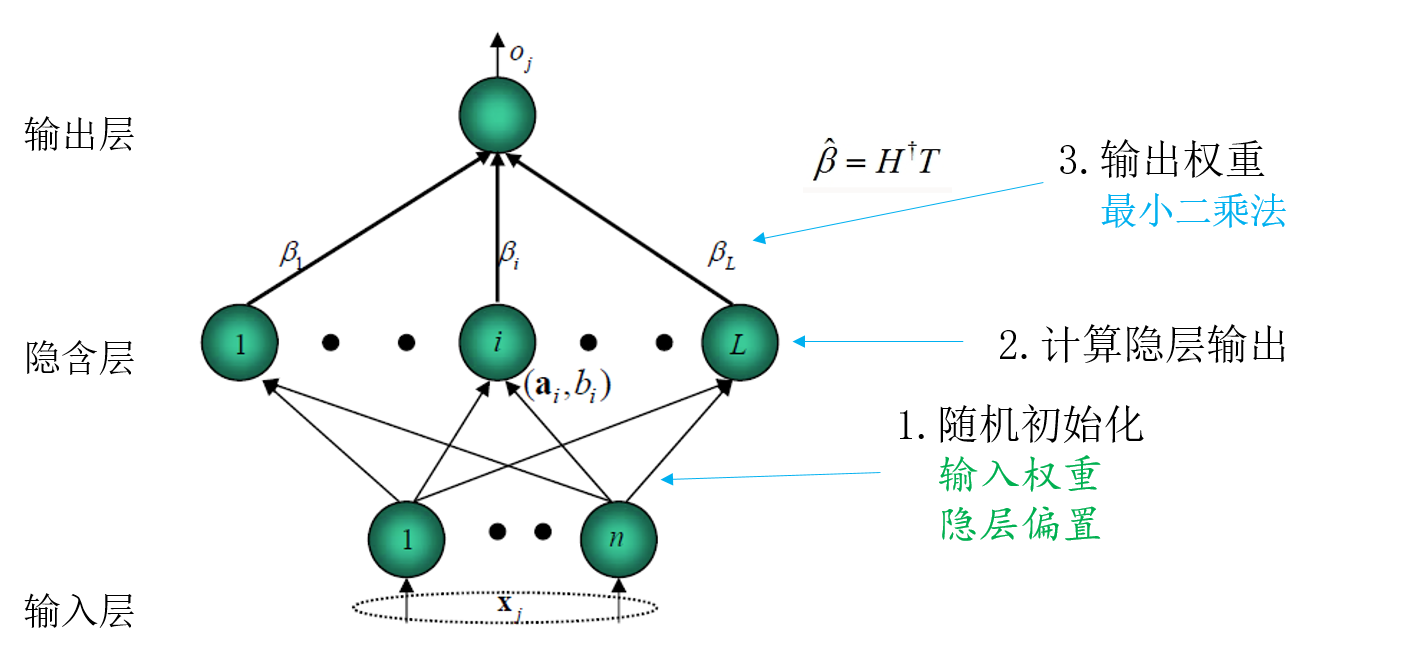
\includegraphics[width=0.7\textwidth]{ch1-ELM.png}
 \caption{超限学习机的网络结构(单隐层前馈型)和算法流程}\label{fig:elm}
\end{figure}

由于没有迭代过程,因此ELM在解决分类或者回归等问题时学习时间很短,主要耗时在矩阵的加减乘除和求逆运算的时间。从学习过程可以看出,ELM的求解思路和最优化方法以及最小二乘辨识算法有些相似,因此基本算法存在的问题和改进思路也类似。上述算法\ref{alg.elm}介绍的是原始ELM的批处理形式,由于实际中样本可能不是一次性获得的,因此和最小二乘算法一样,得到ELM的递推形式,即在线序列ELM算法(OS-ELM)\upcite{LiangHuang2006}。

OS-ELM的推导过程不再详细介绍,和RLS类似。OS-ELM对于控制系统的辨识十分有用,因为控制系统的数据大多是实时产生的,需要在线辨识。然而OS-ELM和批处理形式最后的效果是一致的,只是中间过程不一样,并没有对网络结构和目标函数进行优化。基本ELM优化的仅仅是经验损失风险,目标函数见\eqref{eq:4.nn.cost},因此ELM和OS-ELM都可能存在泛化能力不足和过拟合的现象。为了解决这个问题,相关学者\upcite{Escandell2011,HuynhWon2011}提出了正则化ELM(简称Re-ELM)和正则化OS-ELM(简称ReOS-ELM)。

神经网络在人工智能领域一直发挥重大作用,而人工智能的发展也一直推动着神经网络的研究。为了更好地利用神经网络实现预测和分类,特别是2012年之后,深度学习(Deep learning, DL),借助于大量数据的驱动,在图像分类、语音识别、自然语言处理等应用领域中获得了巨大成功\upcite{ZhengChenZhang2014}。目前大部分深度学习算法都是基于神经网络建立。对于深度学习来说,隐含层的数量级为十几层到几百层不等,甚至上千层。深层网络结构和特征学习思想是深度学习的两大主要特点。针对大数据的应用,超限学习机也有相关变体,如H-ELM(
High-performance extreme learning machine)\upcite{AkusokBjork2015}与深度学习相比。超限学习机在不丢失精度的条件下具有快速的优势,比较见表\ref{tab:elm-dl}所示。可以看出,超限学习机不管是在一般量级的数据样本还是在大数据学习应用领域都具有很大的潜力。
\begin{table}
\centering
\caption{超限学习机与常见深度学习算法的性能比较}\label{tab:elm-dl}
\begin{tabular*}{0.9\textwidth}{@{\extracolsep{\fill}}lccc}
\toprule
算法名称	&测试精度($\%$)	&训练时间 \\
\midrule
H-ELM	&$99.14$	&281.37s\\
Multi-layer ELM	&$99.03\pm0.04$	&281.37s\\
Deep Belief Networks(DBN)	&$98.87$	&20580s(5.7 hours)\\
Deep Boltzmann Machine(DBM)	&$99.05$	&68246s(19 hours)\\
Stacked Auto Encoders(SAE)	&$98.6$	&>17 hours\\
Stacked Denoising AutoEncodes(SDAE)	&$98.72$	&>17 hours\\
\bottomrule
\end{tabular*}
\end{table}

\subsection{ELM估计}
基于机器学习的辨识与建模是数据驱动的,可以适用于线性和非线性系统,主要建立系统的输入输出模型。快速、高精度的特点使得ELM迅速称为系统与控制领域很好的建模、估计与预测算法\upcite{LiJiaLiu2014}。特别是经过优化、提高泛化等方面性能的ELM变体算法,如Re-OSELM。不同于\eqref{eq:4.nn.cost}和\eqref{eq:4.nn.H-T},ReOS-ELM最小化目标的损失函数是
\begin{equation}\label{eq:4.re.cost}
\|\bm{H}\bm{\beta}-\bm{T}\|^{2}+\lambda\|\bm{\beta}\|^{2}
\end{equation}
正则化因子$\lambda$的引入提高了网络的泛化能力。图\eqref{fig.reoselm}展示了用Re-OSELM建立非线性模型的框图。

\begin{figure}[!htb]
  \centering
  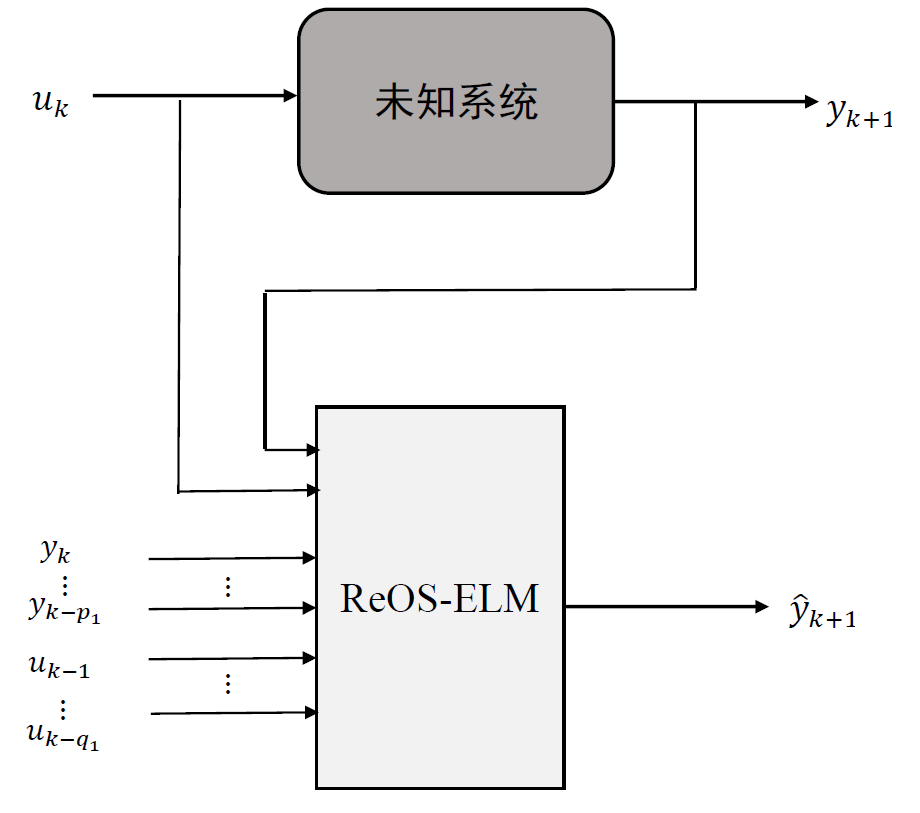
\includegraphics[width=0.6\textwidth ]{ch4-re-elm-c.png}\\	 % e.g.,[scale=0.75], [width=0.75\textwidth ]
  \caption{Re-OSELM算法的建模示意框图}
  \label{fig.reoselm}
\end{figure}

类似于RLS,OS-ELM和Re-OSELM等算法在系统建模与估计过程一般都是分为两个阶段。第一个阶段是初始化网络参数和输出权重$\bm{\beta}$估计值。对于Re-OSELM来说,需要一部分的离线输入输出数据用来完成初始化阶段,通过网络得出$\bm{H}_{0}$和$\bm{T}_{0}$之后,需要计算
\begin{equation}
\begin{split}%
\bm{P}_{0}&=(\bm{H}_{0}^{\tau}\bm{H}_{0}+\lambda \bm{I}_{N_{h}})^{-1}\\
\bm{\beta}^{0}&=\bm{P}_{0}\bm{H}_{0}\bm{T}_{0}
\end{split}
\end{equation}
这里,$\bm{I}_{N_{h}}$是$N_{h}\times N_{h}$的单位矩阵。

在Re-OSELM算法更新权重的过称中引入恰当的或者自适应的遗忘因子$\rho$,可以使得算法能够应用到时变参数系统中。由于正则化因子$\lambda$的存在,即使不需要大于隐含层个数的样本数据用来初始化$\bm{\beta}^{0}$,初始小规模的训练集也是比不可少的。然而,在控制系统中,由于输出值跟实际输入密切相关,因此一定数量的离线输入输出数据一般情况下是难以获得的,这就限制了Re-OSELM在实际控制系统中的应用。

ITF-OELM(Initial-training-free online extreme learning machine)算法\upcite{GaoWongWong2016}就是用来解决缺少离线初始化数问题而提出的。ITF-OELM算法主要针对下面的单输入单输出离散时间非线性系统
\begin{equation}\label{eq:4.siso}
y_{k+1} = g(\bm{x}_{k})+\phi(\bm{x}_{k})u_{k}
\end{equation}
这里$\bm{x}_{k}$是由$\{u_{k},y_{k}\}$组成的回归向量,$g(\cdot)$和$\phi(\cdot)$是具有未知参数的未知非线性函数。用ITF-OELM算法分别估计$g(\cdot)$和$\phi(\cdot)$,得到其相应的估计值$\hat{g}(\cdot)$和$\hat{\phi}(\cdot)$,那么基于ITF-OELM估计的自适应控制律为
\begin{equation}\label{eq:4.itf.u}
u_{k}=\frac{y_{k+1}^{*}-\hat{g}(\bm{x}_{k})}{\hat{\phi}(\bm{x}_{k})} 
\end{equation}
这里,$y_{k+1}^{*}$是期望的输出值。

基于ITF-OELM的自适应控制框图如图\ref{fig.itf-oelm}所示。ITF-OELM算法与Re-OSELM的不同点主要在于初始化输出权重的过程。前者不需要一定数量的离线数据,仅仅用第一组到达的数据初始化估计。另外,ITF-OELM还引入了再学习机制,即如果发现估计偏差较大,就重新初始化网络的所有参数,重新学习。这样,ITF-OELM可以应用于快时变系统,且不需要过多的离线数据。
\begin{figure}[!htb]
  \centering
  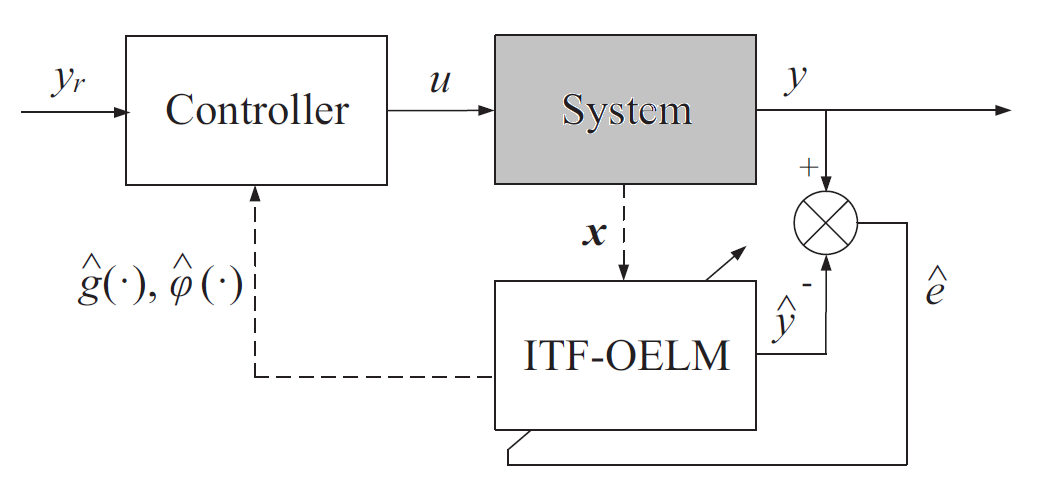
\includegraphics[width=0.7\textwidth ]{ch4-itf.png}\\	 % e.g.,[scale=0.75], [width=0.75\textwidth ]
  \caption{基于ITF-OELM的自适应控制框图}
  \label{fig.itf-oelm}
\end{figure}

下面借助ITF-OELM来解决本课题的非参数部分的估计问题。首先要确定的是网络的输入输出样本数据。本文要估计的非线性部分为
\begin{equation}
z_{k} = f(\bm{\psi}_{k}) + \epsilon_{k+1}
\end{equation}
因此,神经网络的输入是$d_{2}=p_{2}+q_{2}$维向量
$$\bm{\psi_{k}}=[y_{k},y_{k-1},\ldots,y_{k-p_{2}},u_{k-1},\dots,u_{k-q_{2}+1}]^{\tau}$$
$d_{2}$的具体数值视实际被控对象而定。输出是标量$z_{k}$。因此网络的输出层只有一个神经元,输入层含$d_{2}$个神经元。

本课题针对半参数系统在原始的ITF-OELM算法基础上做了两点变化。一方面是估计的非线性函数只有一个,另一方面是在线学习机制的不同。训练网络采用的输入数据$\bm{\psi}_{k}$直接来源于输入和观测到的历史输出数据,然而输出样本数据为
\begin{equation}\label{eq:4.hatz}
\hat{z}_{k-1}=y_{k}-u_{k-1}-\bm{\phi}_{k}^{\tau}\hat{\bm{\theta}}_{k-1}
\end{equation}
这个非线性估计部分是实际测量结果$y_{k}-u_{k-1}$除去参数估计之后的剩余部分。用基于单隐层网络的ELM学习算法得到的估计值是
\begin{equation}\label{eq:4.z.breave}
\breve{z}_{k}=H_{k}\beta^{k}
\end{equation}

和其他监督学习算法一样,网络的训练结果依赖于样本数据的准确性。$\hat{z}_{k-1}$的值依赖于参数估计值$\hat{\theta}$,因此当参数估计值趋于稳定或者参数集合收敛到一定范围之后,需要重新初始化网络参数,继续辨识。也就是说,本课题在实施ITF-OELM算法时,不直接采用原本的再学习机制,而是引入另外一种情况下的再学习机制。这样就可以做到非参数估计更加准确。

本课题基于ELM算法估计非参数部分的实施过程依赖和控制密切相关,故具体算法公式将和自适应控制器设计一起在下一节介绍。

\section{自适应控制器}\label{sect:4.3}
\begin{figure}[!htb]
  \centering
  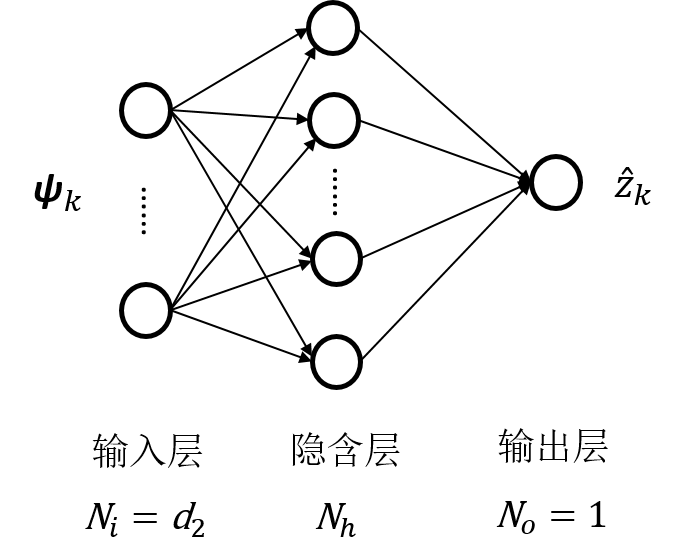
\includegraphics[width=0.55\textwidth]{ch4-elm-use.png}\\	 % e.g.,[scale=0.75], [width=0.75\textwidth ]
  \caption{半参数自适应控制系统中采用的单隐层前馈网络结构和参数}
  \label{fig.elm.use}
\end{figure}

\subsection{算法设计}\label{sect:4.3.1}
用信息浓缩估计参数部分,用ELM估计非参数部分,如图\ref{fig.elm.use}。在前面两种算法的基础上,可以设计出半参数自适应控制器\upcite{ZhouMaLiYang2017},主要包含两个过程,即初始化阶段和自适应控制阶段。在初始化阶段,需要完成信息浓缩估计器关联先验信息设置相关参数集的任务,以及ELM学习算法的网络参数初始化任务;自适应控制阶段前半段主要是参数估计,后半段主要是神经网络的学习更新非参数部分的估计,从而产生合适的控制输入,完成轨迹跟踪任务。

控制的目标是使得系统\ref{eq:4.semi-u}跟踪上期望的轨迹$y^{*}_{k},\ k\geq0$。下面介绍具体实施流程,其中信息浓缩估计部分直接针对二维参数情形设计。

\begin{enumerate}%
%1
\item \textbf{初始化阶段}
\begin{enumerate}%
%1.1
\item 设置$k=0$,系统的初始状态为
\begin{equation*}
\begin{split}%
\phi_{0}&=[y_{0},\ y_{-1}]^{\tau}\\
\psi_{0}&=[y_{0},\dots,,y_{-p_{2}},u_{-1},\dots,u_{-q_{2}+1}]
\end{split}
\end{equation*}
\item 根据关于$\bm{\theta}$的先验信息可以得到初始的多边形为$\Gamma_{0}$(通常是四边形),以及初始的参数估计$\hat{\bm{\theta}}_{0}$.
\item 定义SLFN网络的隐含层神经元个数$N_{h}$,正则化因子$\lambda$和遗忘因子$\rho$.
\item 对于第$i$个隐层神经元,随机初始化网络参数$(a_{i},b_{i})$,$i=1,2,\ldots,N_{h}$.
\item 设置$\beta^{0}$和$P_{0}$为
\begin{equation}\label{eq.elm0}
\begin{split}%
& P_{0} = (\lambda \bm{I_{N_{h}}})^{-1} \\
& \beta^{0} = \bm{0}_{N_{h}}
\end{split}
\end{equation}
这里,$\bm{I_{N_{h}}}$和$\bm{0}_{N_{h}}$分别记作$N_{h}\times N_{h}$的单位矩阵和$N_{h}\times1$的零向量。
\item 设置再学习机制参数。让$\sigma_{k}=var(C_{k})$代表在多边形区域$C_{k}$的所有顶点坐标的方差,即
\begin{equation}
\begin{split}%
\sigma_{n_{k}}(1) &= var(X_{P_{1}},X_{P_{2}},\ldots,X_{P_{n_{k}}}) \\
\sigma_{n_{k}}(2) &= var(Y_{P_{1}},Y_{P_{2}},\ldots,Y_{P_{n_{k}}})
\end{split}
\end{equation}
\item 设置$Flag=0$,意味着尚未激活再学习过程,并记$\delta$为学习方差的上限。
\item 随机产生一个有界的控制输入$u_{0}$,并发送给控制系统\eqref{eq:4.semi-u};设置$k=1$,然后转到Step 2(a).
\end{enumerate}
%2
\item \textbf{自适应控制阶段}
\begin{enumerate}%
%2.a
\item 获得系统在第$k$个时刻的输出值$y_{k}$,并利用第二章的公式\eqref{eq:2.v}计算$v_{k,1}$和$v_{k,2}$.
%2.b
\item 用第三章的公式得到当前的多边形区域$C_{k}$,并将$C_{k}$的中心作为当前参数估计值$\hat{\bm{\theta}}_{k}$.
%2.c
\item 计算$\sigma_{k}$,如果$Flag=0\bigwedge\sigma_{k}(1)\leq\delta\bigwedge\sigma_{n_{k}}(2)\leq\delta$ 那么设置$\gamma=1$与$Flag=1$.
%2.d
\item 设置$\hat{z}_{k-1}=y_{k}-\phi_{k-1}^{\tau}\hat{\bm{\theta}}_{k}-u_{k-1}$.
%2.e
\item 如果$\gamma=1$那么执行(i); 否则,执行(ii).
\begin{enumerate}%
\item Updating:将$(\bm{\psi}_{k-1},\hat{z}_{k-1})$作为SLFN的输入输出样本数据,计算网络的隐含层输出$H_{k-1}$,并使用下面的等式计算矩阵$P_{k}$和隐含层到输出层的权重
\begin{equation}\label{eq.elmk}
\begin{split}%
P_{k}=&\frac{1}{\rho}(P_{k-1}-P_{k-1}H_{k-1}^{\tau}(\rho+H_{k-1}P_{k-1}H_{k-1}^{\tau})^{-1}H_{k-1}P_{k-1})\\
\beta^{k}=&\beta^{k-1} + P_{k-1}H_{k-1}^{\tau}(\hat{z}_{k-1}-H_{k-1}\beta^{k-1})
\end{split}
\end{equation}
\item Relearning:执行在初始化阶段的步骤1-(c),1-(d),1-(e).
\end{enumerate}
\item 将$\bm{\psi}_{k}$作为SLFN的输入向量,并计算隐含层的输出矩阵$H_{k}$,从而得到非参数的估计
\begin{equation}\label{eq.hat.z.k}
\breve{z}_{k}=H_{k}\beta^{k}
\end{equation}
\item 结合参数和非参数两部分的估计,根据必然等价原理设计控制输入为
\begin{equation}\label{eq.4:u}
u_{k}=y^{*}_{k+1}-\phi_{k}^{\tau}\hat{\bm{\theta}}_{k}-\breve{z}_{k}
\end{equation}
\item 设置$k=k+1$,然后转到Step 2(a).
\end{enumerate}
\end{enumerate}

\subsection{稳定性分析}\label{sect:4.3.2}
下面针对系统\ref{eq:4.semi-u}和半参数自适应控制算法分析闭环特性。系统在$k+1$时刻的期望输出为$y^{*}_{k+1}$,实际输出值为$y_{k+1}$,则跟踪误差定义为
\begin{equation}
e_{k+1} = y_{k+1} - y^{*}_{k+1}.
\end{equation}
从方程\eqref{eq:4.semi-u}, \eqref{eq:4.hatz}和\eqref{eq.4:u},容易得到
\begin{equation}\label{eq:4.stab}
\begin{split}%
e_{k+1} & = y_{k+1} - y^{*}_{k+1}\\
& = y_{k+1} - \hat{y}_{k+1} + \hat{y}_{k+1} - y^{*}_{k+1}\\
& = (y_{k+1} - \phi_{k}^{\tau}\hat{\theta}_{k} - \breve{z}_{k} - u_{k} )+(\phi_{k}^{\tau}\hat{\theta}_{k} + \breve{z}_{k} + u_{k}  - y^{*}_{k+1})\\
& = \phi_{k}^{\tau}\theta_{k} + z_{k} - \phi_{k}^{\tau}\hat{\theta}_{k} - \breve{z}_{k}\\
& = \phi_{k}^{\tau}(\theta_{k} - \hat{\theta}_{k}) + (z_{k} - \breve{z}_{k})\\
& = \phi_{k}^{\tau}\tilde{\bm{\theta}}_{k}+\tilde{z}_{k}
\end{split}
\end{equation}
从上面的方程\eqref{eq:4.stab}可以看出,如果参数部分和非参数部分的估计误差$\tilde{\bm{\theta}}_{k}$和$\tilde{z}_{k}$收敛到零,那么跟踪误差$e_{k+1}$也收敛到零。前面一章设计的信息浓缩估计可以保证未知参数估计收敛到零,并且本章的ELM估计非参数部分也可以保证收敛性,因此,本章设计的半参数自适应控制器可以保证渐进稳定性。

\section{仿真实例}\label{sect:4.4}

\subsection{仿真环境}\label{sect:4.4.1}
本章验证自适应控制器的性能,选择仿真如下半参数被控对象
\begin{equation}\label{eq:4.plant}
y_{k+1} = \theta_{1}y_{k} + \theta_{2}y_{k-1} + u_{k} + f(y_{k},y_{k-1}) + \epsilon_{k+1} 
\end{equation}
其中,系统的未知参数和未知函数设定为
\begin{equation}
\begin{array}{c}
\theta_{1} = -1\textbf{, }\theta_{2} = 1\\
f(y_{k},y_{k-1}) = \sin(y_{k}^{2}) + \cos(y_{k-1})
\end{array}
\end{equation}
同时,未知的噪声序列是独立同分布(i.i.d)的随机有界均匀分布,取自$U(-0.1,0.1)$。该被控对象的参数部分是二维情形,非参数部分也是二维情形,即$p_{1}=2$且$q_{2}=2$。系统可利用的先验信息在数学上描述为
\begin{equation}\label{eq.4:aprior}
\begin{split}
&\underline{f}(\psi_{k})=-3,\ \overline{f}(\psi_{k})=4\\
&\underline{\epsilon}=-0.1,\ \overline{\epsilon}=0.1\\
&\underline{\theta}_{1}=-10,\ \overline{\theta}_{1}=10\\
&\underline{\theta}_{2}=-10,\ \overline{\theta}_{2}=15
\end{split}
\end{equation}

为了更好的验证半参数自适应控制器的性能,本章选取了经典的自适应控制算法,即自校正控制器(STR)作为对比算法。自校正控制器(或者自校正调节器)采用递推最小二乘算法(RLS)估计未知参数。不过由于RLS针对的是线性系统,而本章要控制的对象是\eqref{eq:4.plant}是非线性的。对比仿真实验的唯一控制变量在于自适应控制算法,因此先验信息\eqref{eq.4:aprior}对于STR同样可以利用,需要对原生的RLS估计进行简单的改进,补偿掉非线性部分。

对比方法RLS实际估计的线性部分为
\begin{equation}\label{eq:4.zrls}
L_{k}\triangleq\theta_{1}y_{k} + \theta_{2} y_{k-1}=y_{k+1}-u_{k}-\hat{z}_{RLS}
\end{equation}
其中,$\hat{z}_{RLS}$是STR实施过程中对非线性部分的一个粗略估计,用来补偿掉非线性部分,具体值可取
\begin{equation}\label{eq:4.zhatrls}
\hat{z}_{RLS}=\frac12 (\underline{f}(\psi_{k})+\overline{f}(\psi_{k})) 
\end{equation}
RLS估计算法也包括两个过程,第一个是初始化过程确定初始值,即
\begin{equation}\label{eq:4.rls.0}
\begin{split}
&\bm{\pi}_{0}=\alpha \bm{I}_{d_{1}}\\
&\bm{\theta}^{0}=[0.1,\dots,0.1]^{\tau}
\end{split}
\end{equation}
$\alpha$取较大的数(一般为$10^{4}$到$10^{8}$之间)。第二阶段是递推过程,每一步都会改变$\bm{\theta}$和$\bm{\pi}^{0}$的值。根据递推最小二乘算法,第$k$时刻的估计为
\begin{equation}\label{eq:4.rls.k}
\begin{split}
\hat{\bm{\theta}}_{k}&=\hat{\bm{\theta}}_{k-1}+ \zeta_{k} \bm{\pi}_{k-1} \bm{\phi}_{k} (L_{k}-\bm{\phi}_k^\tau \bm{\theta}_{k-1})\\
\zeta_k&=(1+\bm{\phi}_{k}^{\tau} \bm{\pi}_{k-1} \bm{\phi}_{k})^{-1}\\
\bm{\pi}_{k}&=\bm{\pi}_{k-1}-\zeta_k \bm{\pi}_{k-1} \bm{\phi}_{k} \bm{\phi}_{k}^{\tau} \bm{\pi}_{k-1}
\end{split}
\end{equation}
方程\eqref{eq:4.zhatrls}到\eqref{eq:4.rls.k}就是本章对比仿真采用的RLS算法。

\subsection{仿真结果}\label{sect:4.4.2}
设定的期望跟踪信号\upcite{ZhouMaLiYang2017}为
\begin{equation}\label{eq:4.sim.yd}
y_{k}^{*} = 1.5\sin(2\bm{\pi} k\times T_{s})
\end{equation}
其中,控制周期为$T_{s}=0.01$s。仿真半参数自适应控制和自校正控制算法,得到系统的输出曲线分别为\ref{fig.sim.elm.sys}和\ref{fig.sim.str.sys}。在图\ref{fig.sim.elm.sys}中,可以看出半参数自适应控制的轨迹跟踪精度比较好,系统的实际输出很快的跟踪上了期望的输出,误差逐渐收敛到一个很小的范围。相反,自校正控制的跟踪效果就较差,经过一段时间后,系统的实际输出和期望值偏差仍然较大,如图\ref{fig.sim.str.sys}所示。在本节的仿真实例中,自适应控制的输出跟踪误差在自校正控制的基础上减少了大约10倍。
\begin{figure}[!htb]
	\centering
	\subfigure[输出轨迹]{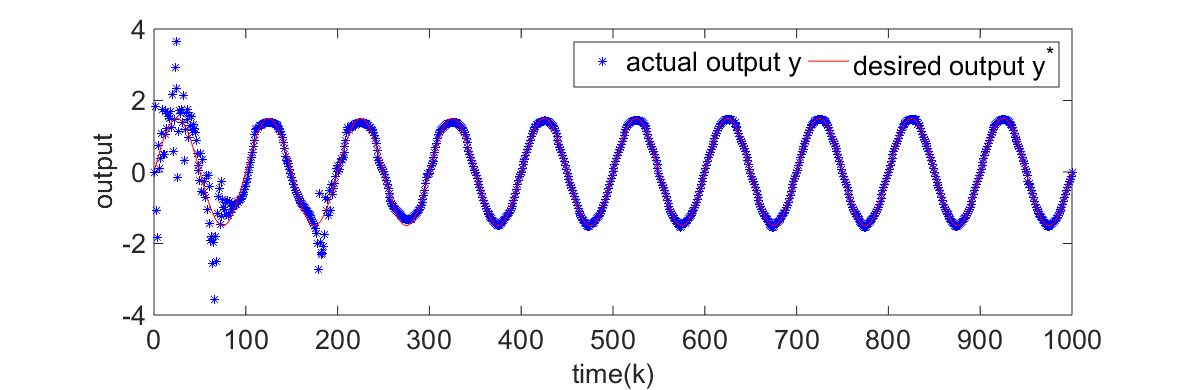
\includegraphics[width=0.65\textwidth ]{ch4-sim-elm-y.png}\label{fig.sim.elm.y}}\\
	\subfigure[跟踪误差]{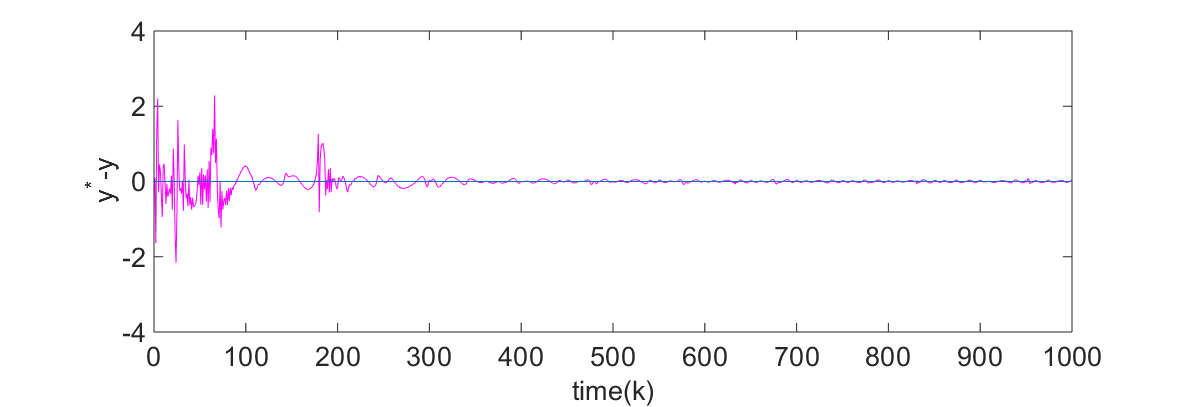
\includegraphics[width=0.65\textwidth ]{ch4-sim-elm-yerror.png}\label{fig.sim.elm.ye}}
	%\subfigure[控制输入]{\includegraphics[width=0.5\textwidth ]{ch4-sim-elmu.png}\label{fig.sim.elm.u}}
	\caption{系统输出结果:半参数自适应控制算法}
	\label{fig.sim.elm.sys}
\end{figure}

\begin{figure}[!htb]
	\centering
	\subfigure[输出轨迹]{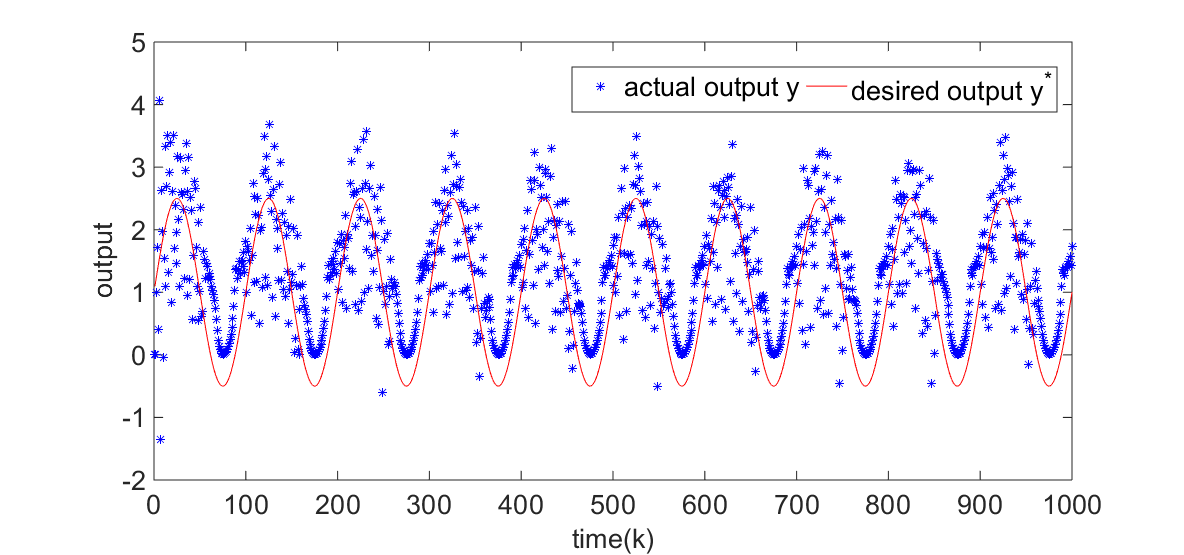
\includegraphics[width=0.65\textwidth ]{ch4-sim-str-y.png}\label{fig.sim.str.y}}\\
	\subfigure[跟踪误差]{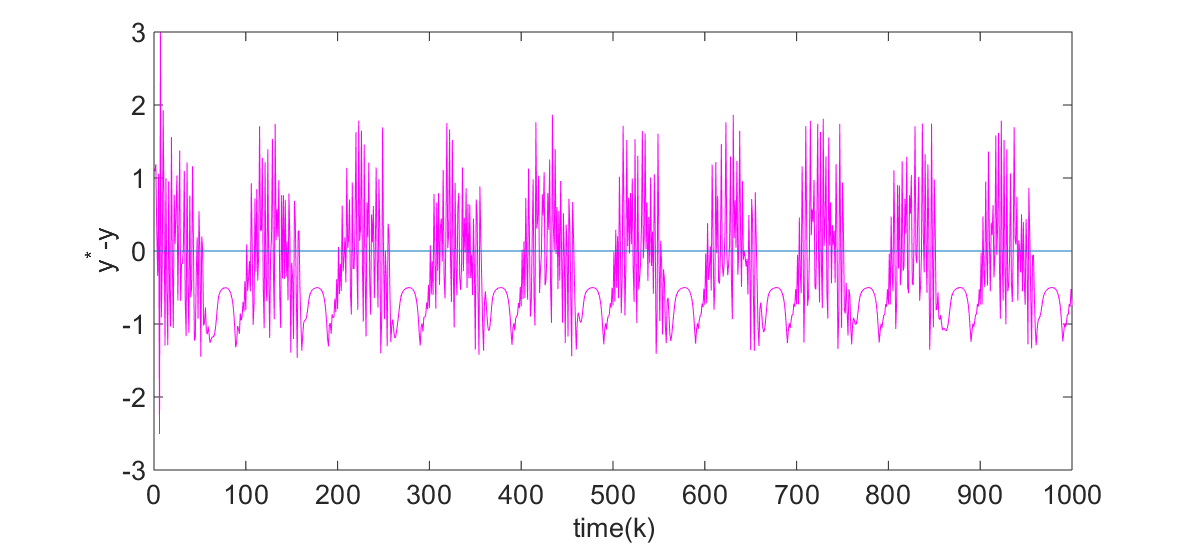
\includegraphics[width=0.65\textwidth ]{ch4-sim-str-yerror.png}\label{fig.sim.str.ye}}
	%\subfigure[控制输入]{\includegraphics[width=0.5\textwidth ]{ch4-sim-elmu.png}\label{fig.sim.elm.u}}
	\caption{系统输出结果:修改的自校正控制算法}
	\label{fig.sim.str.sys}
\end{figure}

造成跟踪控制效果较大差异的重要原因之一,就是两种控制算法中对系统参数估计算法的不同,图\ref{fig.sim.str.sys}展示了仿真得到的参数估计曲线。相对于图\ref{fig.sim.str.theta}中改进的最小二乘算法来说,图\ref{fig.sim.elm.theta}的信息浓缩估计参数估计比较准确。

除了对系统参数不确定性的处理外,半参数自适应控制中用在线超限学习机估计非参数部分,估计结果如图\ref{fig:4.sim.elm.f},选择了径向基函数作为激活函数,网络的隐含层个数在10到20之间。从图中可以,对非线性函数的逼近结果很好,导致对下个周期的非参数部分估计比较准确。这充分说明引入超限学习机这种机器学习算法之后大大减少了系统的非参数不确定性,从而能够计算出合适的控制输入,给到被控对象。另外,基于超限学习机的网络学习过程也没有影响控制的实时性,计算很快,在普通PC机上(实验计算机配置为Intel i5处理器,主频为2.3GHz)每个周期的估计时间在0.05毫秒以内,如果系统经过裁剪和优化可进一步提高运算速度,基本能够满足基于工业PC的控制系统对实时性的要求。网络学习过程并没有引入一般深度网络依赖的并行计算等复杂设计,在普通的工业嵌入式系统中即可实现。

\section{本章总结}\label{sect:4.5}
本章主要设计了基于超限学习机的非线性估计和半参数自适应控制。首先给出了半参数系统的轨迹跟踪问题的数学描述,并分析了半参数模型的自适应估计和控制问题;然后介绍了超限学习机的主要思想、算法特点和改进算法,并用合适的超限学习机变体算法设计了非参数部分的估计算法;接着在信息浓缩和超限学习机的自适应估计基础上,设计了针对半参数系统轨迹跟踪问题的自适应控制器,并分析了闭环跟踪稳定性;最后用仿真实例验证本章设计的半参数自适应控制算法的性能,和改进的自校正控制算法进行对比测试。本章选择的研究模型对后面的实际应用有较强的指导意义。

\begin{figure}[!htb]
	\centering
	\subfigure[信息浓缩估计]{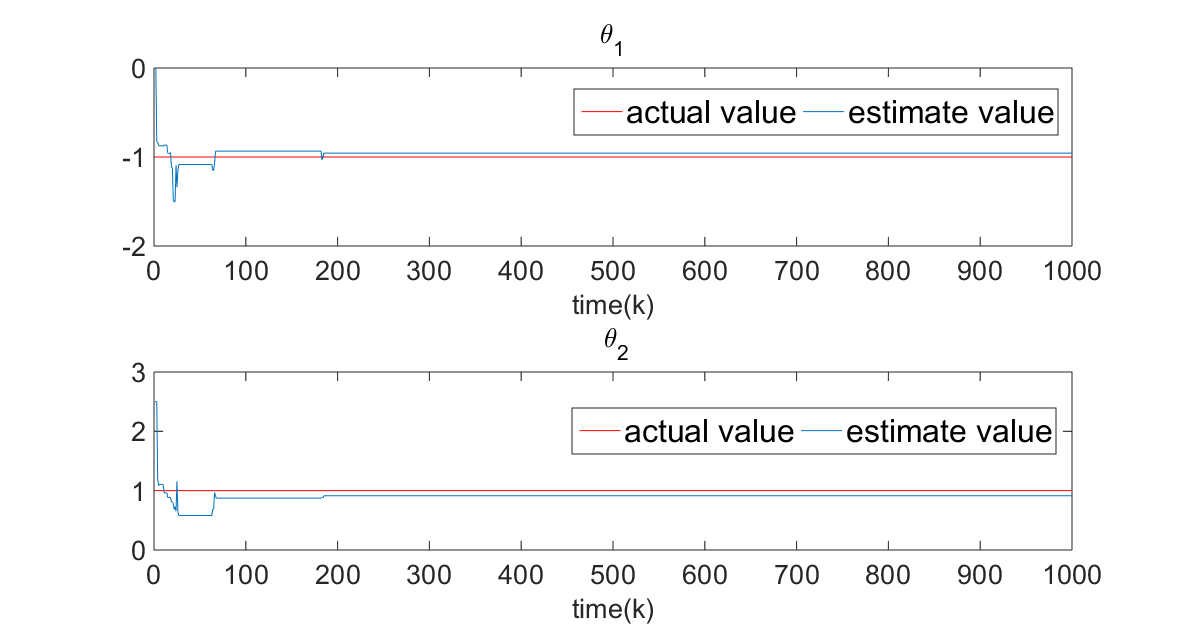
\includegraphics[width=0.65\textwidth ]{ch4-sim-elm-theta.png}\label{fig.sim.elm.theta}}\\
	\subfigure[改进的最小二乘估计]{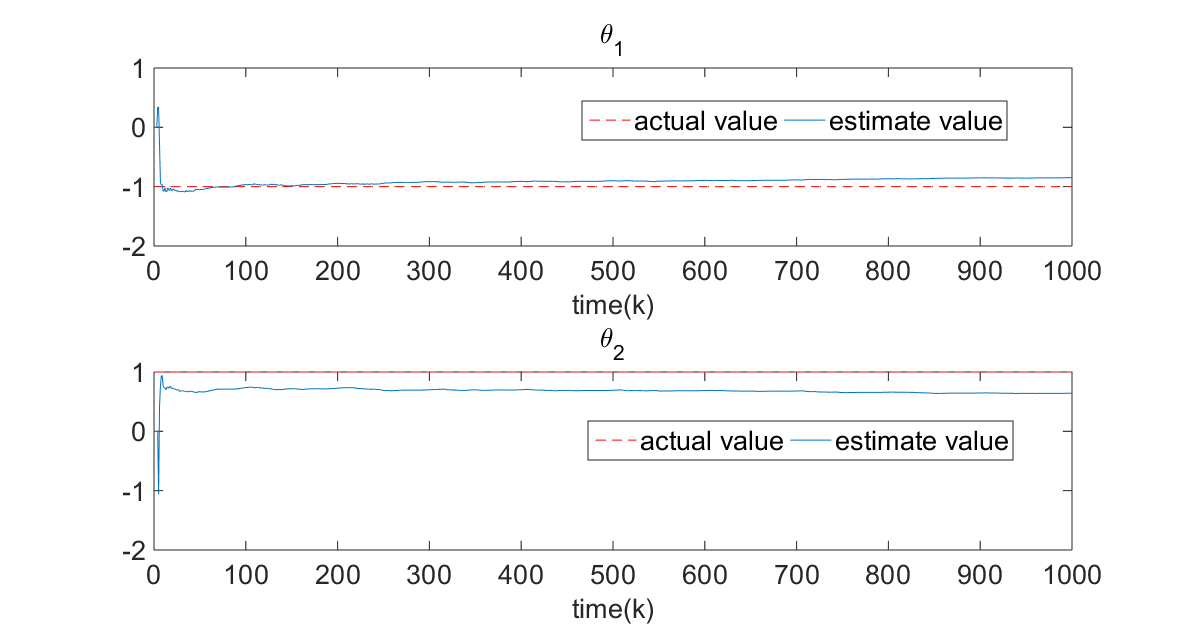
\includegraphics[width=0.65\textwidth ]{ch4-sim-str-theta.png}\label{fig.sim.str.theta}}
	\caption{未知参数估计结果对比}
	\label{fig.sim.str.sys}
\end{figure}

\begin{figure}[!htb]
  \centering
  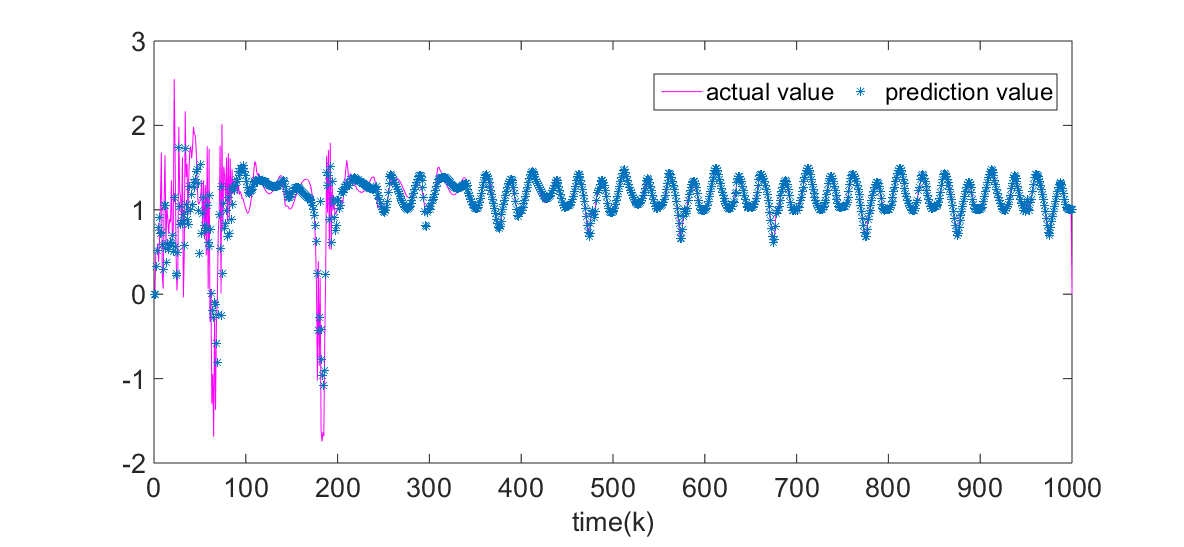
\includegraphics[width=0.65\textwidth ]{ch4-sim-elm-f.png}\\
% e.g.,[scale=0.75], [width=0.75\textwidth ]
  \caption{半参数自适应控制中超限学习机对非参数部分的估计结果}
  \label{fig:4.sim.elm.f}
\end{figure}
%%==================================================
%% chapter5.tex for BIT Master Thesis
%% version: 0.1
%% last update: Nov 8th, 2017
%%==================================================
\chapter{半参数自适应运动控制}\label{chap:5}
反馈控制是为解决实际问题而研究设计的。前面几章针对一种典型先验信息和数学描述的模型设计了半参数自适应估计与控制器,并用数值仿真验证了控制器性能。本章将考虑半参数自适应控制引入到运动控制场景,解决多关节机械臂中伺服电机的控制问题。
\section{问题描述}\label{chap:5.1}
\subsection{机器人控制}\label{5.1.1}
21世纪以来,机器人技术被认为是对未来新兴产业发展具有重要意义的高技术之一。一般来说,机器人是一个复杂的多输入、多输出非线性系统,具有时变、强耦合和非线性的动力学特征\upcite{TanWang2013}。机器人运动学和动力学的非线性和耦合性使得机器人控制系统的设计十分复杂。一般来说,将如图\ref{fig.robot}所示机器人(机械臂)的运动控制分成两个阶段分别优化,即任务空间的轨迹(路径)规划和关节空间的跟踪控制\upcite{ShinMckay1986}。前者轨迹(路径)规划部分性能的提高涉及到运动学甚至障碍物约束等多种综合因素的考量,轨迹规划器最终会以关节空间形式给后者(跟踪控制器)提供一段期望的轨迹。本章主要考虑关节空间的跟踪控制问题。

\begin{figure}[!htb]
	\centering
	\includegraphics[width=0.35\textwidth ]{ch5-ur-robot.png}\\	 % e.g.,[scale=0.75], [width=0.75\textwidth ]
	\caption{一种模块化、多关节、协作型的机器人}
	\label{fig.robot}
\end{figure}

工程应用中由于建模和测量的不准确,加上负载的变化以及外部扰动的影响,实际上难以获得机器人精确完整的运动学模型\upcite{LiuJinKun2008}。因此机器人的控制系统中存在的不确定性因素主要可以分为两类,第一类是参数不确定性,如负载质量、连杆长度、连杆质心等物理量全部或部分未知;第二类是非参数不确定性,如高频未建模动态,包括驱动器动力学、结构共振模式,以及低频难以建模动态,如动态/静态摩擦力、关节柔性等。

工业应用的机器人大多具有六个自由度,如图\ref{fig.robot}是自主研制的模块化、多关节、协作型机器人,分别由六个关节J1到J6的执行机构实现。在无障碍情形下,理论上该机器人的末端可以实现空间任意的位姿,其精度主要表现在任务空间(某个笛卡尔空间)的定位精度。工业高性能的应用场合中,一般要求机器人能达到毫米级的定位精度。机器人的位置控制问题最终要驱动各个关节的电机运动,然后经过减速器等传动机构来实现,伺服电机的运动控制与定位精度是影响机器人末端定位精度的关键因素。

\subsection{伺服电机控制}\label{chap:5.1.2}
目前大多数科研、教学和工业应用的机器人都是电力驱动的,一般可分为电压控制和电流控制两种。永磁同步交流伺服电机驱动已成为高性能伺服系统的主要发展方向。对于中小功率型机械臂(比如图\ref{fig.robot}所示的协作机器人)的电机建模来说,一般考虑电流控制情形,即电机具有如下的数学模型\upcite{LvMaster2013}:
\begin{equation}\label{eq:5.motor}
\begin{array}{c}
i_{c} = K_{a}*u_{c}\\
\tau = K_{m} * i_{c}\\
J_{0}\dot{w} + B \omega + \tau_{f}(\omega) + \tau_{l} = K_{m} K_{a} u_{c}
\end{array}
\end{equation}
其中,$Q$、$\omega$和$\dot{\omega}$分别是电机输出的角位移(单位是rad)、角速度(单位是rad/s),角加速度($\mathbf{rad/s^{2}}$);$J_{0}$是折算到电机侧的所有转动惯量之和(包括传动机构和连杆耦合值等,单位是$\mathbf{kg\cdot m^{2}}$);$B$是粘滞摩擦系数(单位是$\mathbf{N\cdot m\cdot s}$),$\tau_{f}$是Coulomb摩擦力矩(单位是$\mathbf{N\cdot m}$);$K_{a}$和$K_{m}$分别是驱动放大器的导纳系数和电机的力矩常数。

机器人多个关节同时运动时,从单个电机侧感受到的惯量$J_{0}$是时变的。虽然理论上可以通过机器人的动力学模型计算出关节侧的转动惯量值,但是前面一节介绍的不确定性因素的存在,惯量值的计算常常不准确,并且计算十分耗时。不过,经过减速器的传动,从电机侧感受到的关节侧转动惯量时变的效应减小。以一般机器人最大功率的第二个关节J2为例(减速比$G$一般为50到150之间),记该轴在机器人动力学模型中惯性矩阵所对应的值为$M_{22}$,则该轴电机侧感受到的所有转动惯量之和为
\begin{equation}\label{eq:5.J0}
J_{0} = J_{m} + \frac{1}{G^{2}}M_{22}
\end{equation}
可以看出,$M_{22}$的变化效应被缩小了$10^{4}$的数量级。然而即使这样,$J_{0$}的准取值依然难以获得。

上述伺服电机的控制输入可以认为是给定电压(本质是控制输入电流),被控的输出量是角位移或者速度。由于电机一般都是高转速、低转矩特性,并且安装位置有时和轴不在同一个地方,因此为了让电机真正驱动每个轴的运动,还需要经过减速器、皮带轮等传动机构将转速变小,同时放大转矩。除了转动惯量的不确定性外,受传动机构间隙等因素的影响,后面的摩擦力项也和角速度等具有是非线性的关系,难以精确建模。如果忽略Coulomb摩擦力矩项,借助于拉普拉斯变换,可以得到电机模型\eqref{eq:5.motor}的传递函数表述式为:
\begin{equation}\label{eq:5.trans}
\frac{\Omega(s)}{U_{c}(s)}=\frac{K_{m}K_{a}}{J_{0}s+B}
\end{equation}
其中$\Omega(s)$和$U_{c}(s)$分别是时域函数$\omega(t)$和$u_{c}(t)$的拉普拉斯变换结果。

方程\eqref{eq:5.trans}是对于速度控制是一阶模型。不过,由于机器人最终控制的是角位移,也就是速度的积分值。因此伺服电机系统可以近似为二阶线性模型,可以采用一些常规的线性控制方法,不过它的参数$J_{0}$时变,$B$常常难以知道精确值。现代伺服系统大都采用数字化离散时间控制。记采样周期为$T_{s}$,从离散时间控制角度,在第$k$个时刻电机的输入量和输出量分别记为
$$u_{k}=u_{c}(k\cdot T_{s}),\ y_{k}=\omega(k\cdot T_{s})$$
则系统\eqref{eq:5.motor}的输入输出关系可以写作
\begin{equation}\label{eq:5.nonlinear}
y_{k+1}=F(\bm{\Psi}{k},\epsilon_{k+1})
\end{equation}
其中$\bm{\Psi}_{k}$是输出$y_{k}$和输入$u_{k}$的历史数据组成的回归向量,$\epsilon_{k+1}$是随机干扰。

方程\eqref{eq:5.nonlinear}综合考虑了Coulomb摩擦等所有未建模动态,这样\eqref{eq:5.motor}转化成离散时间后不确定性大大增加,也就是说电机的离散时间模型本质是非常复杂且难以建立准确建模的,也就给直接控制系统带来了很大困难。实际上,伺服电机系统可以采用常规的线性系统方法如PID控制,可以获得一定的控制效果,但是精度和控制特性都有待提高。这从一个侧面反映了\eqref{eq:5.nonlinear}的主体是线性的,只是线性部分参数可能未知,并且含有难以建模的非参数部分。另外,伺服电机含有大量可利用的先验信息,如电机转矩的有界性、惯量变化的有界性等。这十分符合本课题前面提出的半参数系统特性。

\section{控制器设计}\label{chap:5.2}
基于前面小节的分析,本节将应用半参数模型的理论和方法分析机器人中电机运动控制问题,并设计相应的自适应控制器。
\subsection{半参数建模}\label{5.2.1}
半参数建模的目的在于建立合适的方程(包含线性和非线性部分)去描述实际系统以及蕴含的先验信息。结合方程组\eqref{eq:5.motor},电机的角速度$y_{k+1}$主要取决于上一个时刻的角速度$y_{k}$和加速度$a_{k}$。如果记$\tau_{k}$、$\tau_{k,f}$分别为电流产生的力矩和电机运动的摩擦阻力(即$B \omega + \tau_{f}(\omega)$),则电机在$k$时刻的加速度近似为
$$a_{k}=\frac{(\tau_{k}-\tau_{k,f}-\tau_{l})}{J_{0}}$$
由速度和加速度的微分关系,可以得到电机的角速度$y_{k+1}$为
\begin{equation}\label{eq:5.yk1}
\begin{split}
y_{k+1}&=y_{k}+a_{k}\cdot T_{s}+f'(\bm{\psi}_{k})+\epsilon\\
&=\theta_{1}\cdot y_{k}+\theta_{2}\cdot u_{k}+f(\bm{\psi}_{k})+\epsilon_{k+1}
\end{split}
\end{equation}
其中,$\theta_{1}$未知,可以认为近似为1,而$\theta_{2}$与电机本身参数有关,可以近似为
$$\theta_{2}=\frac{K_{m}K_{a}}{J_{0}}$$
$f(\cdot)$是未知非线性函数,主要融合了难以建模的摩擦和惯量等信息,而$\epsilon_{k+1}$是系的随机干扰。系统的控制输入为电机的电枢电流,即$u_{k}=i_{c}(k\cdot T_{s})$.

在系统\eqref{eq:5.yk1}中,$\bm{\theta}=[\theta_{1},\ \theta_{2}]$是系统的参数不确定性部分,维数
$$d_{1}=p_{1}+q_{1}=1+1=2$$
$$\bm{\phi}_{k}=[y_{k},u_{k}]$$
参数部分的先验信息表现为有界性。$\theta_{1}$近似为1,其先验信息可认为取值在0.8到1.2之间;$\theta_{1}$的上下界可以通过分析电机本身的参数$K_{a}$、$K_{m}$的合适范围,以及在机器人运动过程中惯量$J_{0}$的变化范围等数值确定大致范围。

$f(\bm{\psi}_{k})$是系统的非参数不确定性部分,回归向量$\bm{\psi}_{k}=$是历史输入输出数据的组合,即
$$\bm{\psi}_{k}=[y_{k},\ldots,y_{k-p_{2}},u_{k-1},\dots,u_{k-q_{2}+1}]$$
维数$d_{2}=p_{2}+q_{2}$不定,对应的是网络的输入层神经元个数,一般为1到10之间。一般来说,维数$d_{2}$越大,网络训练的数据越多,则逼近效果越好;但同时,过大的维数也会加重网络训练的计算量,还会造成过拟合,实际中可以调整选择合适的维数。

系统的非参数不确定性部分的先验信息也表现为有界性。由于离散时间化导致这里的$f(\cdot)$难以直接找到它的变化范围,与前面第三章和第四章的上下界函数有所不同。不过,由于电机本身功率、机械条件和加速度的制约,电机的速度与前一个时刻相差不会很大,往往在一定范围内波动,可以认为$f(\bm{\psi}_{k})$关于回归向量$\bm{\psi}_{k}$满足Lipschitz条件。具体表现为,对于两个不同的时刻$k$和$s$,$k\neq s$,存在正常数$L_{f,1}>0$和$L_{f,2}>0$,使得
\begin{equation}\label{eq:5.flim}
\begin{array}{c}
|f(\bm{\psi}_{k})-f(\bm{\psi}_{s})|\leq \Delta_{k,s}\\
\Delta_{k,s}=L_{f,1}\cdot\|\bm{\psi}_{y,k}-\bm{\psi}_{y,s}\|+L_{f,2}\cdot\|\bm{\psi}_{u,k}-\bm{\psi}_{u,s}\|
\end{array}
\end{equation}
$\|\cdot\|$记为向量的某种范数,一般为欧几里得范数。$\bm{\psi}_{y,k}$和$\bm{\psi}_{u,k}$分别是$f(\cdot)$的自变量$\bm{\psi}_{k}$中$y_{k}$和$u_{k}$的向量部分,而由于控制输入$u_{k}$和输出$y_{k}$可能在数量级上并不匹配,因此这里分别采用两个常数$L_{f,1}$和$L_{f,2}$来刻画。

一般来说,随机干扰序列$\epsilon_{k}$也具备有界性且独立同分布,在电机系统中一般取自某个随机均匀分布。关于随机干扰的先验信息为
$$\underline{\epsilon}\leq\epsilon_{k}\leq\overline{\epsilon}.$$

\subsection{自适应估计}\label{5.2.2}
为了实现半参数自适应控制,首先得设计自适应估计算法。由于半参数系统\eqref{eq:5.yk1}的参数部分也是二维情形,非参数部分也是有界的,可以利用其先验信息\eqref{eq:5.flim}借助设计信息浓缩算法估计未知参数。只是有所不同的是,非参数部分的有界形式有所不同,导致算法\ref{alg.ic.2d}和方程\eqref{eq:2.v}中关于直线的参数$v_{k,1}$和$v_{k,2}$的计算有所不同。下面给出具体推导过程。

当$k\geq2$,对于任意$0\leq s\leq k-2$,由约束关系\eqref{eq:5.flim}可以得到
\begin{equation}\label{eq:5.flim.s}
|f(\bm{\psi}_{k-1})-f(\bm{\psi}_{s})|\leq \Delta_{k-1,s}
\end{equation}
而
\begin{equation*}
\begin{split}%
|f(\bm{\psi}_{k-1})-f(\bm{\psi}_{s})|&=(y_{k}-\bm{\theta}^{\tau}\bm{\phi}_{k-1})-(y_{s+1}-\bm{\theta}^{\tau}\bm{\phi}_{s})\\
&=(y_{k}-y_{s+1})-\bm{\theta}^{\tau}(\bm{\phi}_{k-1}-\bm{\phi}_{s})
\end{split}
\end{equation*}
再结合\eqref{eq:5.flim.s}得到
\begin{equation}\label{eq:5.}
|\bm{\theta}^{\tau}(\bm{\phi}_{k-1}-\bm{\phi}_{s})-(y_{k}-y_{s+1})| \leq \Delta_{k-1,s}
\end{equation}
因此进一步得到线性约束不等式组
\begin{equation}\label{eq:5.theta.lim}
(y_{k}-y_{s+1})-\Delta_{k-1,s}\leq\bm{\theta}^{\tau}(\bm{\phi}_{k-1}-\bm{\phi}_{s})\leq\Delta_{k-1,s}+(y_{k}-y_{s+1})
\end{equation}

在几何上,式子\eqref{eq:5.theta.lim}就代表了二维空间中两个半平面的约束,作为每个周期的参数信息集$I_{k}$,可以用来设计信息浓缩估计算法。对于时刻$k-1$,可以和之前每个时刻比较得出一组类似\eqref{eq:5.theta.lim}的不等式约束,那么从理论上说存在$k-2$组。但是考虑到计算量的限制,一般情况下,只需要比较相邻两个时刻即可获得比较充分的信息关系,从而在较短时间内获得未知参数比较准确的估计值$\hat{\bm{\theta}}$。即利用$s=k-2$时的不等式约束
\begin{equation}\label{eq:5.theta.lim}
(y_{k}-y_{k-1})-\Delta_{k-1,k-2}\leq\bm{\theta}^{\tau}(\bm{\phi}_{k-1}-\bm{\phi}_{k-2})\leq\Delta_{k-1,k-2}+(y_{k}-y_{k-1})
\end{equation}

在获得$\bm{\theta}$的估计值之后,则剩余的非参数部分
$$\hat{z}_{k}=y_{k+1}-\hat{\bm{\theta}}^{\tau}\bm{\phi}_{k-1}$$
可以用第四章的基于单隐层神经网络的ITF-OELM算法逼近和预测得到$\breve{z}_{k}$的值。神经网络的输入是包含系统输入和输出历史数据组成的回归向量,实际过程中可以调整相应维度的大小。对于电机模型,一般选择1-3个输出和1-3个控制输入。选择过多的历史数据,也无太大意义,因为运动角度、角速度一般跟加速度、加加速度(有时称之为冲击)关联度较大。

\subsection{控制器设计}\label{5.2.3}
本章要解决的是机器人运动过程中关节空间的角度跟踪控制问题,从轨迹规划器得到伺服电机转动的角度之后,需要作插补运算可以得到电机在每个周期运动的角度、速度和加速度值。本章针对电机运动的角速度,从离散时间角度针对半参数模型\eqref{eq:5.yk1}设计自适应估计与控制律。在离散时间控制中,控制输入只在每个控制周期改变一次,并且只能采用得到每个周期的系统状态变量和观测值,而实际的被控对象是连续时间的模拟量。

通过相关的轨迹发生器可以得到电机在每个运动周期时刻期望的角度$Q_{k}^{*}$、角速度$\omega_{k}^{*}$和角加速度$\dot{\omega}_{k}^{*}$。为了提高伺服电机的定位精度,在电机速度控制的基础上加入位置反馈,将角度跟踪误差作为速度前馈值加入到轨迹规划产生的速度期望值中,即期望的速度跟踪值为
$$y_{k+1}^{*}=\frac{Q_{k}^{*}-Q_{k}}{T_{s}}+\omega_{k+1}^{*}$$
然后对于系统\ref{eq:5.yk1},采用必然等价原理设计的半参数自适应控制律为
\begin{equation}\label{eq:5.uk}
u_{k} = \frac{1}{\hat{\theta}_{1}}(y^{*}_{k+1}-\hat{\theta}_{2}y_{k}-\breve{z}_{k})
\end{equation}

因此,可以得到用半参数自适应控制解决电机伺服控制的总体框图\ref{fig.control.motor}。其中,$Q_{0}$和$Q_{d}$分别为电机的初始角度值和期望的角度值。
\begin{figure}[!htb]
	\centering
	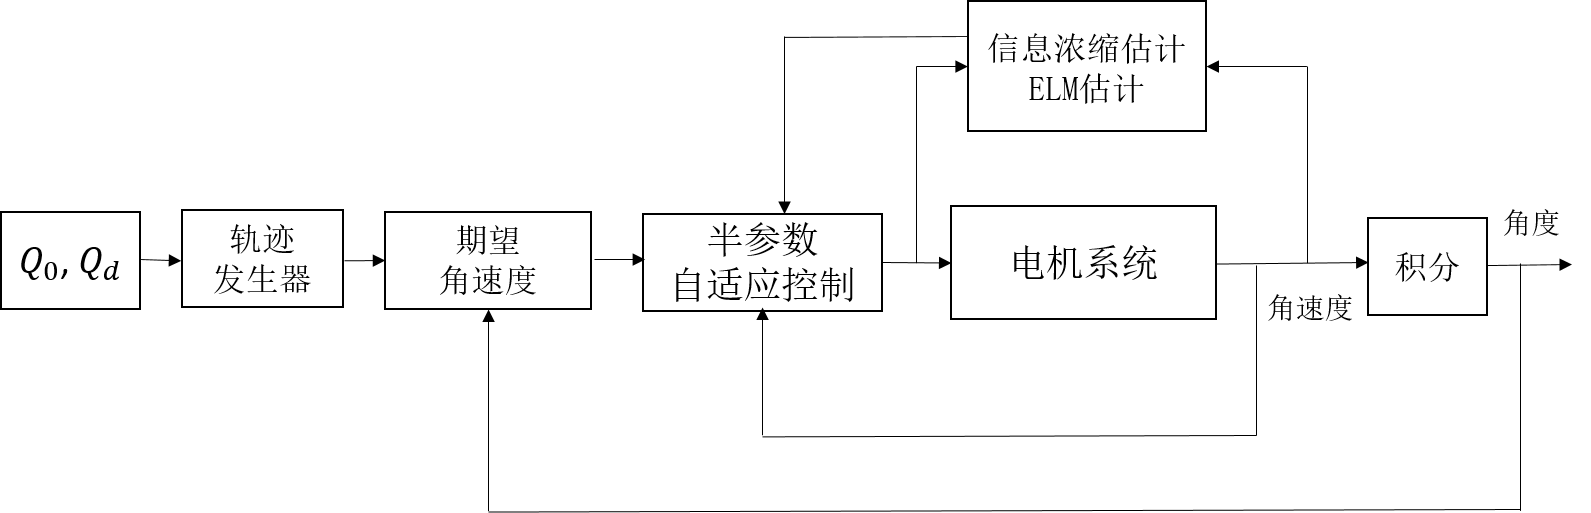
\includegraphics[width=0.85\textwidth ]{ch5-control-fig.png}\\	 % e.g.,[scale=0.75], [width=0.75\textwidth ]
	\caption{基于超限学习机的半参数自适应控制在电机运动控制中的总体框图}
	\label{fig.control.motor}
\end{figure}

\section{仿真实例}
本节以图\ref{fig.robot}所示的机器人第二轴J2安装的伺服电机控制为例验证本章设计的半参数自适应运动控制算法的性能。该伺服电机属于日本松下A6系列全数字式交流伺服电机,具体型号为MHMF022L1V2M,是一种小功率的交流同步电机。相关参数如表\ref{tab:motor}所示。
\begin{table}
\centering
\caption{电机相关参数}\label{tab:motor}
\begin{tabular*}{0.9\textwidth}{@{\extracolsep{\fill}}ll}
\toprule
项目&参数\\
\midrule
额定转矩($N\cdot m$)&0.64\\
最大转矩($N\cdot m$)&2.23\\
额定转速($r\cdot min^{-1}$)&3000\\
额定转速($r\cdot min^{-1}$)&6500\\
额定电流(A)&1.4\\
最大电流(A)&4.3\\
转矩常数$K_{m}$($Nm\cdot A^{-1}$)& 0.4571\\
电机惯量($kg\cdot m^{2}$)&$0.31\times10^{-4}$\\
谐波减速比&120\\
\bottomrule
\end{tabular*}
\end{table}

设定关节轴J2的初始值和期望终值分别为
$$Q_{0}=-45^{o}=0.524rad,\ Q_{d}=85^{o}=1.484rad$$
经过减速器之后,对应的电机角度的初始值和期望终值分别为(弧度制)
$$Q_{0}=-62.88,\ Q_{d}=178.08$$
本章用五次多项式插值作为图\ref{fig.control.motor}的轨迹发生器中的轨迹规划算法,可以做到机器人在关节空间的加速度连续且可导,其导数加加速度(冲击)连续,其轨迹比较平滑\upcite{LiuPhD2009},一般机器人控制器的关节空间的插补都是采用五次多项式进行。在仿真过程中,可以借助于机器人相关工具箱里提供的函数完成插值规划部分。

目前广泛采用的机器人电机驱动通信总线是工业实时以太网EtherCAT,其控制周期一般为0.5ms到10ms之间。为了接近实际情况,本章的电机控制周期取为$T_{s}=1$ms。采用前面设计的半参数自适应控制算法对电机的运动进行轨迹跟踪控制,事先对于电机如表\ref{tab:motor}所示准确参数未知,只是知道大致范围,在这种情况下检验控制性能。最终得到电机系统的输出结果为图\ref{fig.sim.semi.yye},以及过程中的控制输入和非线性部分的估计曲线如图\ref{fig.sim.semi.a}所示。轴2在运动过程中关节角度的跟踪误差平均值为$0.0021$rad。对于如图所示的机器人一般的运动过程中的臂长为1m,则机器人末端的跟踪误差$e_{ac}=0.0021m=2.1mm$,跟踪精度在毫米数量级。

\begin{figure}[!htb]
	\centering
	\subfigure[第二轴的关节运动速度曲线(经过减速器之后)]{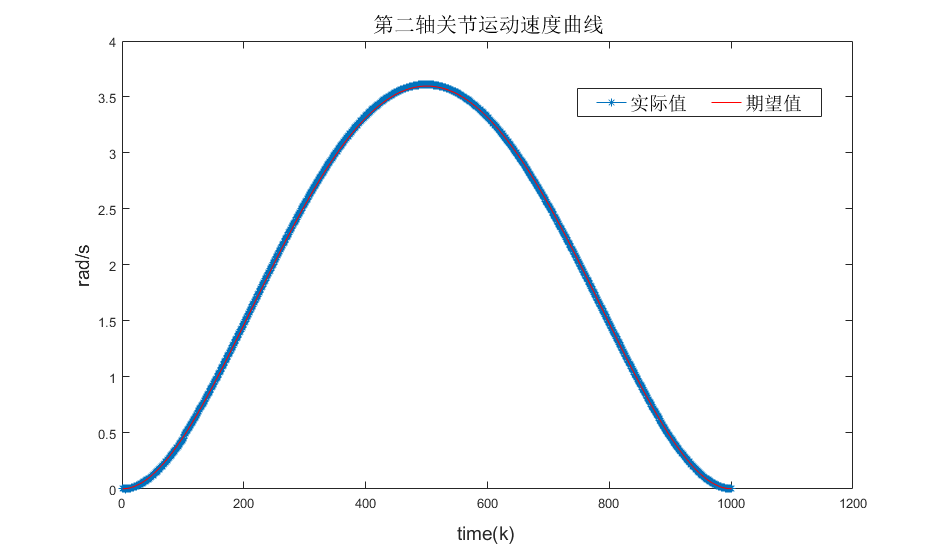
\includegraphics[width=0.65\textwidth ]{ch5-semi-omega.png}\label{fig.sim.semi.y}}\\
	\subfigure[第二轴的关节角位移曲线(经过减速器之后)]{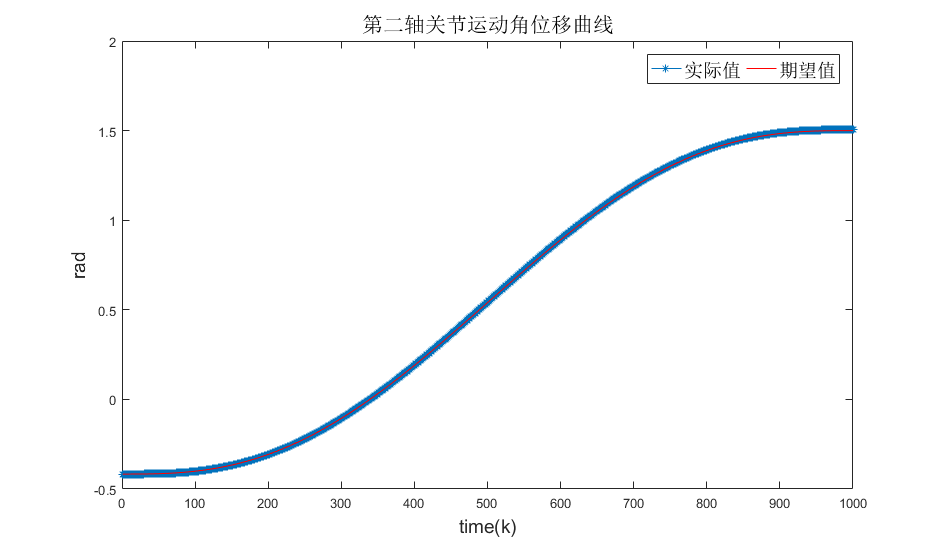
\includegraphics[width=0.65\textwidth ]{ch5-semi-Q.png}\label{fig.sim.semi.ye}}
	%\subfigure[控制输入]{\includegraphics[width=0.5\textwidth ]{ch4-sim-elmu.png}\label{fig.sim.elm.u}}
	\caption{半参数自适应控制算法的系统输出结果,关节角度跟踪误差的平均值为$0.0021$rad}
	\label{fig.sim.semi.yye}
\end{figure}

\begin{figure}[!htb]
	\centering
	\subfigure[第二轴电机系统的非参数部分的估计结果]{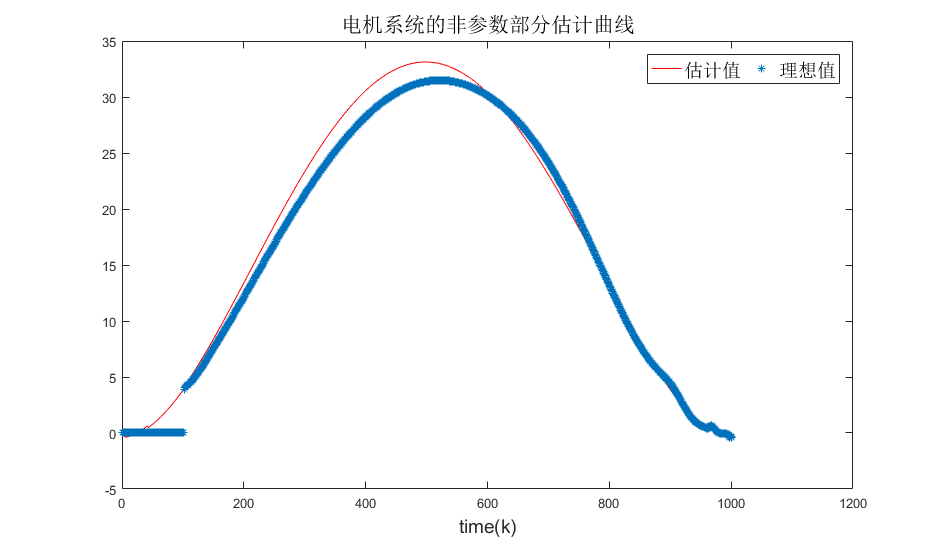
\includegraphics[width=0.65\textwidth ]{ch5-semi-f.png}\label{fig.sim.elm.f}}\\
	\subfigure[第二轴电机系统的控制输入(电机电流)变化曲线]{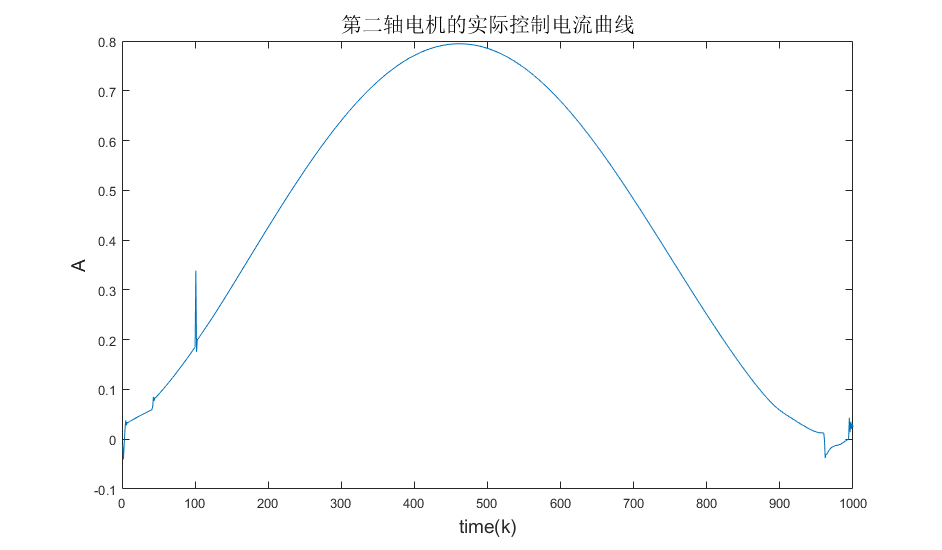
\includegraphics[width=0.65\textwidth ]{ch5-semi-u.png}\label{fig.sim.elm.u}}
	%\subfigure[控制输入]{\includegraphics[width=0.5\textwidth ]{ch4-sim-elmu.png}\label{fig.sim.elm.u}}
	\caption{半参数自适应控制算法的运行和估计特性曲线}
	\label{fig.sim.semi.a}
\end{figure}

另外,采用常规的PID算法进行对比仿真,这里采用的调试PID参数的策略是在电机空载或者小负载以及电机名义标称惯量的情况下调试得到满意的性能,然后加上在机器人负载条件下再次测试。最终得到电机系统的输出结果为图\ref{fig.sim.pid.y},以及过程中的控制输入(电机电流)曲线如图\ref{fig.sim.pid.u}所示。轴2在运动过程中关节角度的跟踪误差平均值为$0.0207$rad。对于如图所示的机器人一般的运动过程中的臂长为1m,则机器人末端的跟踪误差$e_{pid}=0.0207m=2.07cm$,跟踪精度在厘米数量级。
\begin{figure}[!htb]
	\centering
	\subfigure[第二轴的关节运动速度曲线(经过减速器之后)]{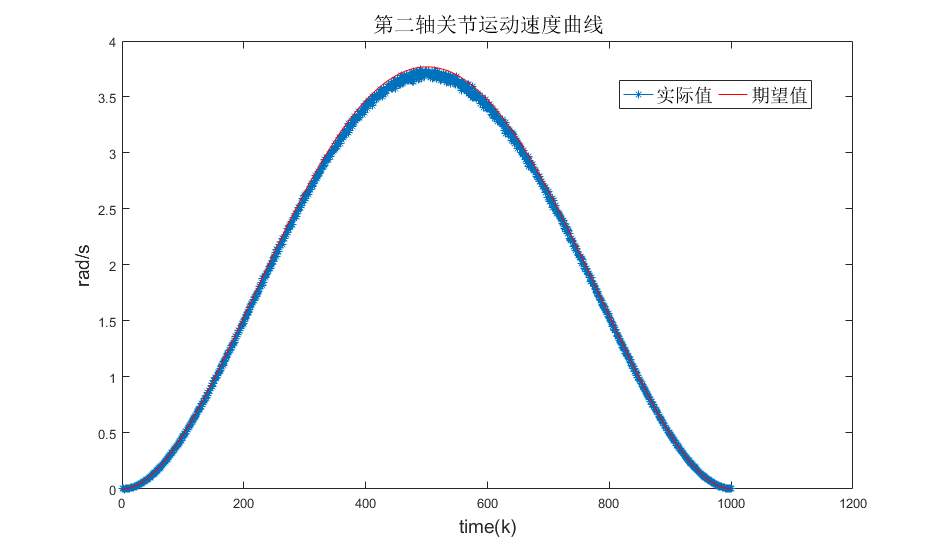
\includegraphics[width=0.65\textwidth ]{ch5-pid-omega.png}\label{fig.sim.pid.y}}\\
	\subfigure[第二轴的关节角位移曲线(经过减速器之后)]{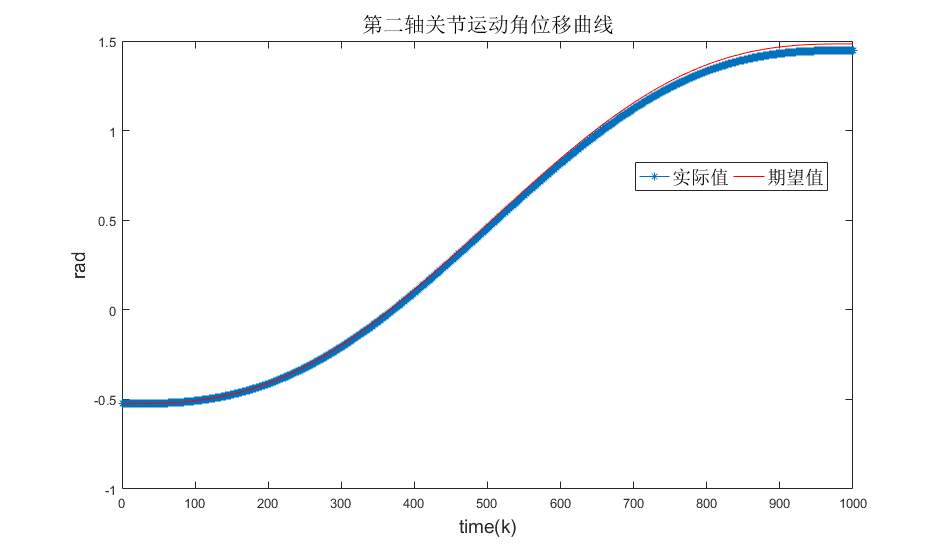
\includegraphics[width=0.65\textwidth ]{ch5-pid-Q.png}\label{fig.sim.pid.ye}}
	%\subfigure[控制输入]{\includegraphics[width=0.5\textwidth ]{ch4-sim-elmu.png}\label{fig.sim.elm.u}}
	\caption{PID控制算法的系统输出结果,关节角度跟踪误差的平均值为$0.0207$rad}
	\label{fig.sim.pid.yye}
\end{figure}

\begin{figure}[!htb]
	\centering
	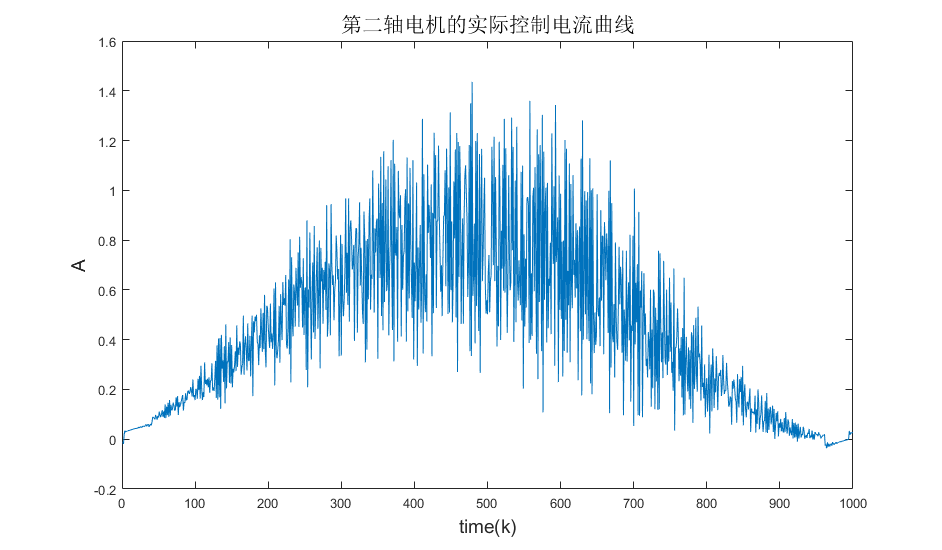
\includegraphics[width=0.5\textwidth ]{ch5-pid-u.png}\\	 % e.g.,[scale=0.75], [width=0.75\textwidth ]
	\caption{PID控制算法中第二轴电机系统的控制输入(电机电流)变化曲线}
	\label{fig.sim.pid.u}
\end{figure}

对比上面两种控制方法结果,可以得出本课题采用基于超限学习机的半参数自适应控制算法对于解决运动控制问题有如下特点:
\begin{enumerate}
\item 基于超限学习机的半参数自适应控制算法提高了系统的跟踪精度,对比常规的PID控制精度可以提高大约一个数量级(10倍)。
\item 基于超限学习机的半参数自适应控制对于系统精度提高主要来源于非参数部分的准确估计,而非参数部分的估计在一定程度也依赖于参数部分的估计。
\item 半参数自适应估计的准确性导致最终的控制输入有比较好的变化曲线,对比图\ref{fig.sim.elm.u}和\ref{fig.sim.pid.u}容易得出。
\end{enumerate}

\section{本章总结}
本章主要将基于超限学习机的半参数自适应估计与控制应用到运动轨迹跟踪控制中,解决机器人运动中电机的控制问题。首先分析了机器人轨迹跟踪和伺服电机运动控制中多种不确定性存在等控制难点;然后应用本课题提出的半参数系统对单轴伺服电机进行了分析和建模;接着设计了基于超限学习机的半参数自适应估计与控制算法应用单轴伺服电机的控制;最后设计了仿真对比实验测试和验证半参数自适应控制的性能。

%%==================================================
%% conclusion.tex for BIT Master Thesis
%% modified by yang yating
%% version: 0.1
%% last update: Dec 25th, 2016
%%==================================================

\begin{conclusion}
系统存在不确定性,一直是控制理论研究和工程应用的难点,特别是在离散时间系统的控制中。本文针对同时具有参数和非参数不确定性的离散时间被控对象,在已有半参数理论的基础上,研究并完善半参数建模、分析、估计与控制方法,充分利用了系统的先验信息和输入输出历史数据,提高了离散时间控制的实时性和准确性。

本文的主要工作总结如下:

1、对反馈控制、非线性控制和自适应控制的发展历程、主要趋势和技术特点进行了系统的归纳和总结,
指出了最小二乘等线性估计方法的不足;研究了人工神经网络在非线性建模与控制中的应用与难点,介绍了超限学习机的算法特点,这是一种在前馈神经网络的实时性应用中具有很大潜力的方法。

2、从回顾反馈机制能力极限等前沿问题出发,针对系统具有参数不确定性和非参数不确定性的特点进行了分析,
将系统分为参数描述的线性部分和非参数描述的非线性部分,概括出了一种半参数建模方法,并对实际系统常用的先验信息进行了数学描述。

3、研究了一种充分利用先验信息的、基于集合的自适应估计方法,即信息浓缩估计,
用于解决半参数系统的参数不确定性部分的估计;设计了二维情形下的具体实现算法和步骤,并在数值仿真实验中测试和验证实际效果;归纳总结了信息浓缩估计算法的优缺点,提出了一些计算复杂度问题的优化方向。

4、介绍了半参数自适应估计与控制问题的一般描述,围绕解决神经网络中经典迭代学习算法的实时性等问题,阐述了超限学习机及其变体的算法特点与非线性建模思路;将超限学习机引入到半参数系统的非参数部分估计中,设计了基于超限学习机的半参数自适应控制算法,并通过仿真实验进行了验证。

5、在机器人与伺服电机等运动体的轨迹跟踪控制中存在大量的不确定性,将基于信息浓缩估计和超限学习机的半参数建模、估计与控制方法应用到机器人场景中伺服电机的控制问题中,对运动控制问题进行了具体设计;在仿真实验中进行算法验证,结果表明半参数自适应控制大大提高了轨迹跟踪精度。

基于超限学习机的半参数自适应控制算法的特点主要体现在,充分利用原有系统的先验信息和输入输出历史数据,结合信息浓缩估计和超限学习机等高效且新颖的算法,其建模与控制思路在解决具有较大不确定性的被控对象时具有一般性与通用性。但是,由于控制中利用的估计算法本身的不足,还有一些问题需要进一步研究与完善:

1、 信息浓缩估计算法的完善。本文目前设计了二维情形下的信息浓缩估计算法,并在自适应运动控制中进行了验证。二维情形可以在一定程度上,解决许多运动控制场景如伺服电机的跟踪控制问题,但是对于涉及到高阶模型,含有多个参数的情况如机器人末端的力反馈控制等问题,可能需要进一步研究高维情形中的信息浓缩估计算法,但基本思路不变。

2、多变量系统的自适应控制实现。本文主要涉及到控制输入和测量输出都是单一变量的情形,多输入多输出情形的建模与分析思路与本文大致相同,只是涉及到更多变量的信息浓缩估计与神经网络计算,可能需要考虑到本文第三章论述的有关计算复杂度相关的优化策略。

3、本文以超限学习机作为非参数部分的估计算法,其出发点在于控制算法的实时性,同时探讨了信息浓缩估计的计算优化问题,这些关键思路对于今后算法移植到工业嵌入式系统打下了很好的基础,因此半参数自适应控制的工业应用问题是本文后续研究的重要工作。

%end of conclusion
\end{conclusion}

%% 参考文献,五号字,使用 BibTeX,包含参考文献文件.bib

%\bibliography{reference/chap1,reference/chap2} %多个章节的参考文献
\bibliography{reference/all}


%%%%%%%%%%%%%%%%%%%%%%%%%%%%%%
%% 后置部分
%%%%%%%%%%%%%%%%%%%%%%%%%%%%%%

%% 附录(章节编号重新计算,使用字母进行编号)
\appendix
\renewcommand\theequation{\Alph{chapter}--\arabic{equation}}  % 附录中编号形式是"A-1"的样子
\renewcommand\thefigure{\Alph{chapter}--\arabic{figure}}
\renewcommand\thetable{\Alph{chapter}--\arabic{table}}

%%%==================================================
%% app1.tex for BIT Master Thesis
%% modified by yang yating
%% version: 0.1
%% last update: Dec 25th, 2016
%%==================================================


\chapter{***}

附录相关内容…
 
%\include{chapters/app2}

%(其后部分无编号)
\backmatter

% 发表文章目录
%%==================================================
%% pub.tex for BIT Master Thesis
%% modified by yang yating
%% version: 0.1
%% last update: Dec 25th, 2016
%%==================================================

\begin{publications}{99}
    \item\textsc{Hao Zhou, Hongbin Ma, Nannan Li, Chenguang Yang}. {Semi-parametric Adaptive Control of Discrete-time Systems Using Extreme Learning Machine}[C].The 9th International Conference on Modelling, Identification, Control, 2017.(EI检索会议)
    \item\textsc{Hao Zhou, Hongbin Ma*, Haiyang Zhan}. {Sampled Adaptive Control for Multi-joint Robotic Manipulator with Force Uncertainties}[C]. Intelligent Robotics, Applications, 2016.(EI检索会议)
    \item\textsc{Hao Zhou, Hongbin Ma*, Dong Wang, Sunjie Chen}. {Stochastic Adaptive Control of Semi-flexible Robotic Manipulator}[C], 2016. 2016 International conference on Advanced Robotics, Intelligent Systems, 2016.(EI检索会议)
    \item\textsc{王冬, 马宏宾, 周浩, 陈孙杰}. {一种基于iBeacon的室内定位系统及方法}[P]. 2016.(发明专利,已受理)
    \item\textsc{王冬, 马宏宾, 周浩, 陈孙杰}. {基于Kinect骨骼追踪和无标定视觉伺服的人机协作系统}[P]. 2016.(发明专利,已受理)
    \item\textsc{王冬, 马宏宾, 周浩, 陈孙杰}. {一种半柔性机械臂系统的控制方法}[P]. 2017.(发明专利,已受理)
\end{publications}

% 致谢
%%==================================================
%% thanks.tex for BIT Master Thesis
%% modified by yang yating
%% version: 0.1
%% last update: Dec 25th, 2016
%%==================================================

\begin{thanks}

本论文的工作是在导师马宏宾教授的指导下独立完成的。两年半的时光匆匆划过,虽有苦有泪,但它始终是我这一生中一段重要的旅程。研究生阶段让我在更好的完善自己的同时,也丰富了我的知识,开阔了眼界。而如今,我能够顺利的完成我的毕业论文,也是因为一直有那些人陪伴在我的左右,在我错误时指导我,在我失意时陪伴我,在我受挫时鼓励我。在此论文完成之际,我要对曾经帮助过我的师长、亲人、同学和朋友表示诚挚的谢意。

感谢敬爱的导师马宏宾教授在我的学习和生活中给与的帮助和教诲。在入学之初,马老师就开始悉心安排我硕士期间的课题方向,给了我一些比较有意思小问题,既有理论上的,也有工程上的,让我首先尝试去解决,给提供了一些基础性的书籍和资料。这些问题的解决使我逐渐进入机器人和自适应控制的研究当中。后来在深入开展课题的研究中,马老师经常与我不断交流。每次遇到一些障碍,马老师总能让我醍醐灌顶,找到一些新的思路。马老师深厚的理论素养、忘我的工作热情和优秀的的人格魅力,以及对学生无微不至的关怀,让我终身受益。

感谢付梦印教授、王美玲教授在学习和科研上的指导,两位老师学识渊博、平易近人使我获益匪浅;感谢周培德老师给我提供和补充其他相关领域的知识和方法;感谢张星红师姐和张晓飞师兄,为我修改论文提供许多宝贵的意见和细节上的指导;感谢陈孙杰、于华超等实验室的同学与我一起探讨学术、工程上的难题,为我提供了许多仿真实验上的有益帮助。

感谢张明阳、白伟和王斌等同学在研究生期间给我的帮助,今后必将怀念与你们一起在自动化学院一起奋斗和生活的日子,特别是那些美好的时光。

在此,我也要特别感谢我的父母及其他亲人朋友,你们的支持和帮助,一直是我前进的动力,能够顺利完成硕士学位,也离不开你们在经济上的支持,感恩你们无私的爱!

最后,感谢本论文中所引用的参考文献的作者,你们的文章给了我无限的启迪和智慧,感谢本论文的评审老师和答辩委员会老师,同时也感谢自动化学院的所有任课教师们,感谢各位老师的批评指正。

\end{thanks}

% 作者简介(博士论文需要)
%%%==================================================
%% resume.tex for BIT Master Thesis
%% modified by yang yating
%% version: 0.1
%% last update: Dec 25th, 2016
%%==================================================

\begin{resume}

本人…。

\end{resume}


\end{document}
